\documentclass[a4paper]{article}
\usepackage{lmodern}
\usepackage{amssymb,amsmath}
\usepackage{ifxetex,ifluatex}
\usepackage{fixltx2e} % provides \textsubscript
\ifnum 0\ifxetex 1\fi\ifluatex 1\fi=0 % if pdftex
  \usepackage[T1]{fontenc}
  \usepackage[utf8]{inputenc}
\else % if luatex or xelatex
  \ifxetex
    \usepackage{mathspec}
  \else
    \usepackage{fontspec}
  \fi
  \defaultfontfeatures{Ligatures=TeX,Scale=MatchLowercase}
\fi
% use upquote if available, for straight quotes in verbatim environments
\IfFileExists{upquote.sty}{\usepackage{upquote}}{}
% use microtype if available
\IfFileExists{microtype.sty}{%
\usepackage{microtype}
\UseMicrotypeSet[protrusion]{basicmath} % disable protrusion for tt fonts
}{}
\usepackage[margin=1in]{geometry}
\usepackage{hyperref}
\hypersetup{unicode=true,
            pdftitle={Distribuição Log-Normal},
            pdfauthor={Luiz Fernando Palin Droubi; Norberto Hochheim; Willian Zonato},
            pdfborder={0 0 0},
            breaklinks=true}
\urlstyle{same}  % don't use monospace font for urls
\usepackage{graphicx,grffile}
\makeatletter
\def\maxwidth{\ifdim\Gin@nat@width>\linewidth\linewidth\else\Gin@nat@width\fi}
\def\maxheight{\ifdim\Gin@nat@height>\textheight\textheight\else\Gin@nat@height\fi}
\makeatother
% Scale images if necessary, so that they will not overflow the page
% margins by default, and it is still possible to overwrite the defaults
% using explicit options in \includegraphics[width, height, ...]{}
\setkeys{Gin}{width=\maxwidth,height=\maxheight,keepaspectratio}
\IfFileExists{parskip.sty}{%
\usepackage{parskip}
}{% else
\setlength{\parindent}{0pt}
\setlength{\parskip}{6pt plus 2pt minus 1pt}
}
\setlength{\emergencystretch}{3em}  % prevent overfull lines
\providecommand{\tightlist}{%
  \setlength{\itemsep}{0pt}\setlength{\parskip}{0pt}}
\setcounter{secnumdepth}{5}
% Redefines (sub)paragraphs to behave more like sections
\ifx\paragraph\undefined\else
\let\oldparagraph\paragraph
\renewcommand{\paragraph}[1]{\oldparagraph{#1}\mbox{}}
\fi
\ifx\subparagraph\undefined\else
\let\oldsubparagraph\subparagraph
\renewcommand{\subparagraph}[1]{\oldsubparagraph{#1}\mbox{}}
\fi

%%% Use protect on footnotes to avoid problems with footnotes in titles
\let\rmarkdownfootnote\footnote%
\def\footnote{\protect\rmarkdownfootnote}

%%% Change title format to be more compact
\usepackage{titling}

% Create subtitle command for use in maketitle
\newcommand{\subtitle}[1]{
  \posttitle{
    \begin{center}\large#1\end{center}
    }
}

\setlength{\droptitle}{-2em}

  \title{Distribuição Log-Normal}
    \pretitle{\vspace{\droptitle}\centering\huge}
  \posttitle{\par}
  \subtitle{Propriedades e aplicações}
  \author{Luiz Fernando Palin Droubi\footnote{SPU/SC,
  \href{mailto:luiz.droubi@planejamento.gov.br}{\nolinkurl{luiz.droubi@planejamento.gov.br}}} \\ Norberto Hochheim\footnote{UFSC,
  \href{mailto:hochheim@gmail.com}{\nolinkurl{hochheim@gmail.com}}} \\ Willian Zonato\footnote{SPU/SC,
  \href{mailto:willian.zonato@planejamento.gov.br}{\nolinkurl{willian.zonato@planejamento.gov.br}}}}
    \preauthor{\centering\large\emph}
  \postauthor{\par}
      \predate{\centering\large\emph}
  \postdate{\par}
    \date{19/09/2018}

\usepackage[brazil]{babel}
\usepackage{graphicx}
\usepackage{float}
\usepackage{subfig}
\usepackage{animate}
\usepackage{caption}
\newcommand{\pkg}[1]{{\normalfont\fontseries{b}\selectfont #1}}
\let\proglang=\textsf
\let\code=\texttt
\usepackage{booktabs}
\usepackage{longtable}
\usepackage{array}
\usepackage{multirow}
\usepackage[table]{xcolor}
\usepackage{wrapfig}
\usepackage{float}
\usepackage{colortbl}
\usepackage{pdflscape}
\usepackage{tabu}
\usepackage{threeparttable}
\usepackage{threeparttablex}
\usepackage[normalem]{ulem}
\usepackage{makecell}

\usepackage{amsmath,amssymb}

\begin{document}
\maketitle

\section*{Resumo}\label{resumo}
\addcontentsline{toc}{section}{Resumo}

Pretende-se com este artigo detalhar o motivo pelo qual a transformação
de variável dependente pela função logaritmo é frequentemente adequada
na área de avaliação de imóveis. Um procedimento muito comum nesta área
é a adoção de transformações para a obtenção de um ``melhor'' modelo de
regressão. A mais usual e preferida de muitos avaliadores é a função
logaritmo, especialmente para a variável dependente. Muitas vezes esta
transformação é adequada e percebe-se uma notória melhora no ajuste do
modelo. Outras vezes, esta transformação pode não ser adequada. Apesar
do modelo aparentar-se melhor ajustado, problemas podem ocorrer quanto
às verificações das hipóteses clássicas da regressão, as quais nem
sempre os avaliadores estão tão atentos quanto estão com as verificações
dos intervalos de confiança e níveis de significância. No entanto, o
avaliador que assim procede estará verificando intervalos de confiança e
níveis de significâncias incorretos, haja vista que a hipótese da
heteroscedasticidade implica na incorreção destas inferências.
Entendemos que a melhor maneira para apresentar aos avaliadores a
importância de criteriosas escolhas de transformações seja através da
análise do histograma da variável original e transformada. Normalmente,
uma boa escolha de transformação leva à uma distribuição aproximadamente
normal. Quando a variável dependente apresenta distribuição lognormal,
esta transformação é a transformação logaritmica. Desta maneira,
demonstramos as características básicas desta distribuição, sua
formulação, características além do seu relacionamento com a
distribuição normal. Por fim, demonstramos as implicações da adoção da
transformação da variável dependente e abordamos o problema da
retransformação da variável dependente à sua escala original.

\section{INTRODUÇÃO}\label{introducao}

A transformação de variáveis é um procedimento comum na Engenharia de
Avaliações. No entanto, a transformação dos dados por vezes é realizada
sem uma análise profunda do comportamento das variáveis. A \emph{Food
and Drug Administration} (FDA), órgão federal dos EUA que atua no
controle da comercialização de alimentos e medicamentos no país,
recomenda:

\begin{quote}
A transformação desnecessária de dados deve ser evitada. Caso tenha sido
realizada transformação de dados, uma justificativa para a escolha da
transformação junto com a interpretação das estimativas dos efeitos do
tratamento com base nos dados transformados deve ser fornecida.(FDA,
\protect\hyperlink{ref-fda}{1988} apud KEENE
(\protect\hyperlink{ref-keene}{1985}))
\end{quote}

No entanto, a transformação logarítmica é especial, por uma série de
aspectos, como pode ser visto em KEENE
(\protect\hyperlink{ref-keene}{1985}).

A distribuição lognormal apresenta diversas aplicações práticas. É
comum, na área de avaliação de imóveis, mas não apenas\footnote{Dados
  estritamente positivos, como valores em moeda, altura, peso, etc,
  normalmente seguem a distribuição lognormal.}, nos depararmos com
dados que seguem esta distribuição. Neste artigo pretendemos demonstrar
as principais características da distribuição lognormal, sua relação com
a distribuição normal de Gauss, assim como debatemos a melhor maneira de
se lidar com dados lognormais.

\section{REVISÃO BIBLIOGRÁFICA}\label{revisao-bibliografica}

\subsection{Formulação}\label{formulacao}

A formulação da distribuição lognormal para os parâmetros \(\mu\) e
\(\sigma\) pode ser vista abaixo (FARIAS)

\[\begin{cases}
f(x;\mu, \sigma) = \frac{1}{x\sigma\sqrt{2\pi}}\exp(-\frac{(log(x) - \mu)^2}{2\sigma^2}) & \forall x > 0 \\ 
0 & \text{ se } x = 0 
\end{cases}\]

\subsection{Propriedades}\label{propriedades}

\subsubsection{Valor Esperado e
Variância}\label{valor-esperado-e-variancia}

O valor Esperado \(\mathbb{E}\) de uma variável aleatória com
distribuição lognormal \(X\) é (FARIAS):

\[\mathbb{E}(X) = \exp \left (\mu + \frac{\sigma^2}{2} \right )\] E sua
variância é:

\[\newcommand{\Var}{\operatorname{Var}} \Var(X) = \exp (2\mu+\sigma^2)(\exp(\sigma^2)-1)\]

\subsubsection{Medidas de Tendência
Central}\label{medidas-de-tendencia-central}

A figura \ref{fig:densidade_medidas} mostra a posição das medidas de
tendência central (moda, média e mediana) para um variável aleatória de
distribuição log-normal.

\begin{figure}[H]

{\centering 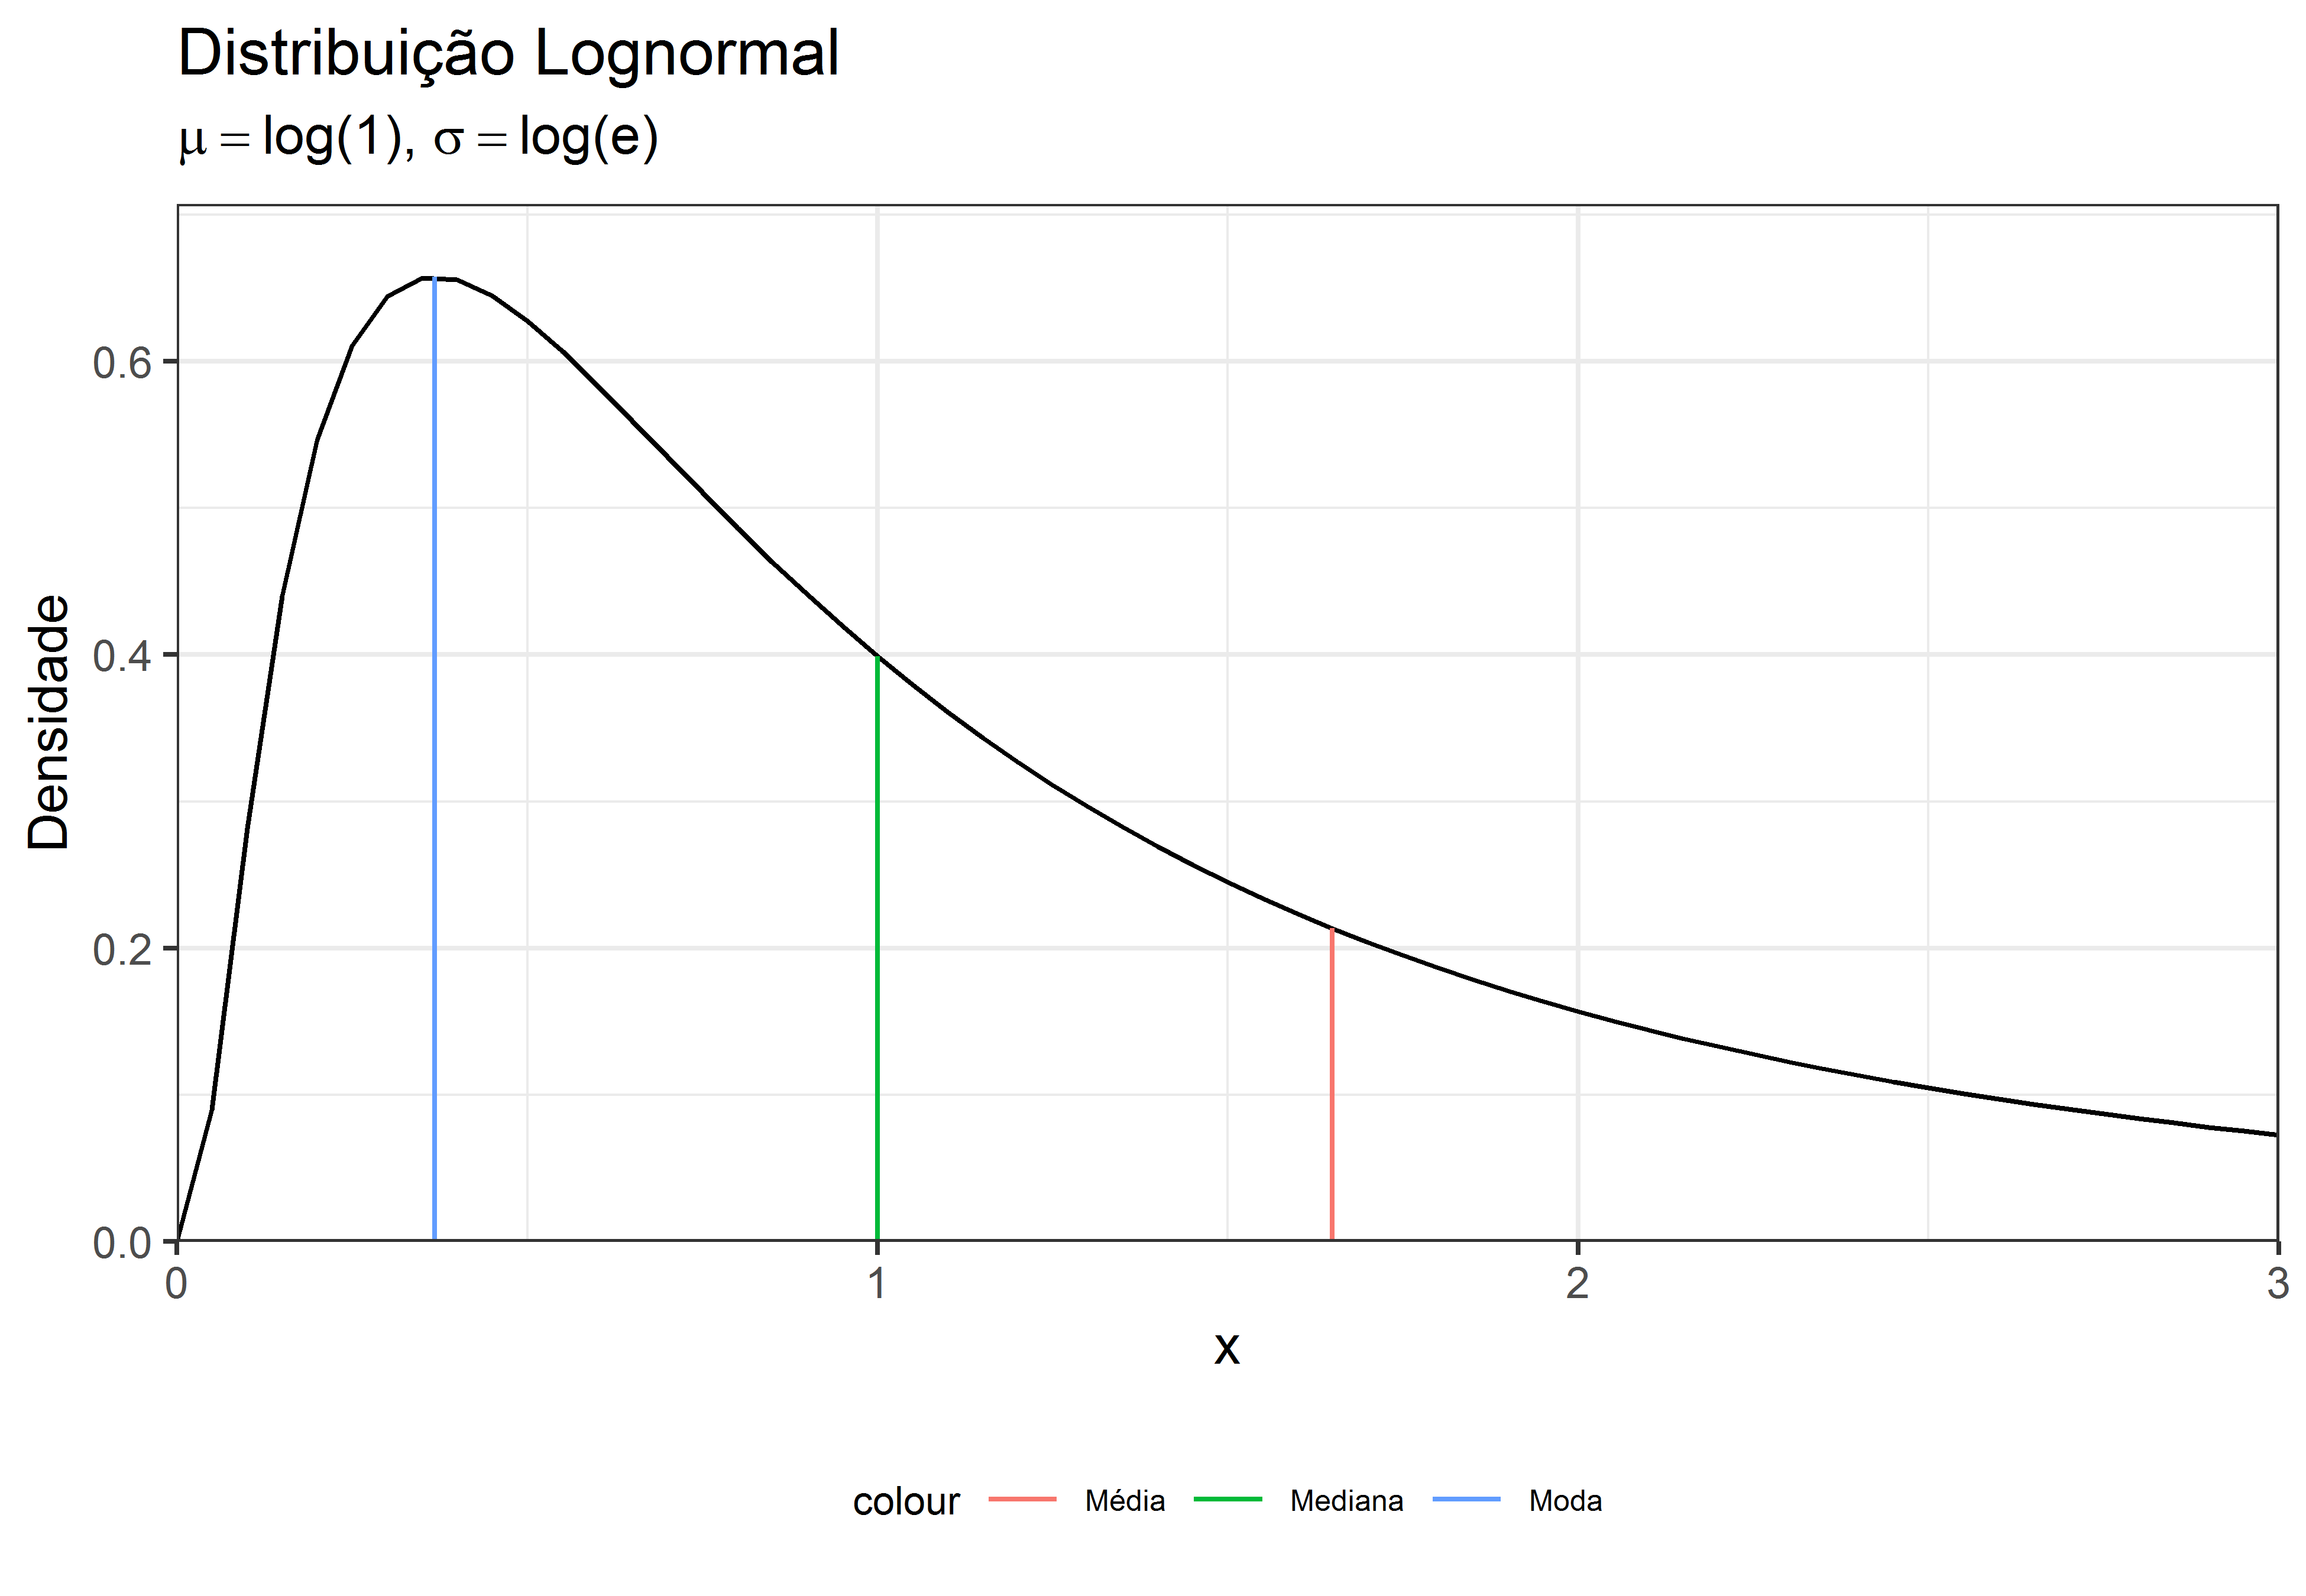
\includegraphics[width=0.5\linewidth]{images/densidade_medidas-1} 

}

\caption{Ilustração das posições de medidas de tendência central numa distribuição lognormal.}\label{fig:densidade_medidas}
\end{figure}

\subsubsection{Efeito das variações do desvio-padrão na forma da
distribuição}\label{efeito-das-variacoes-do-desvio-padrao-na-forma-da-distribuicao}

\begin{figure}[H]

{\centering 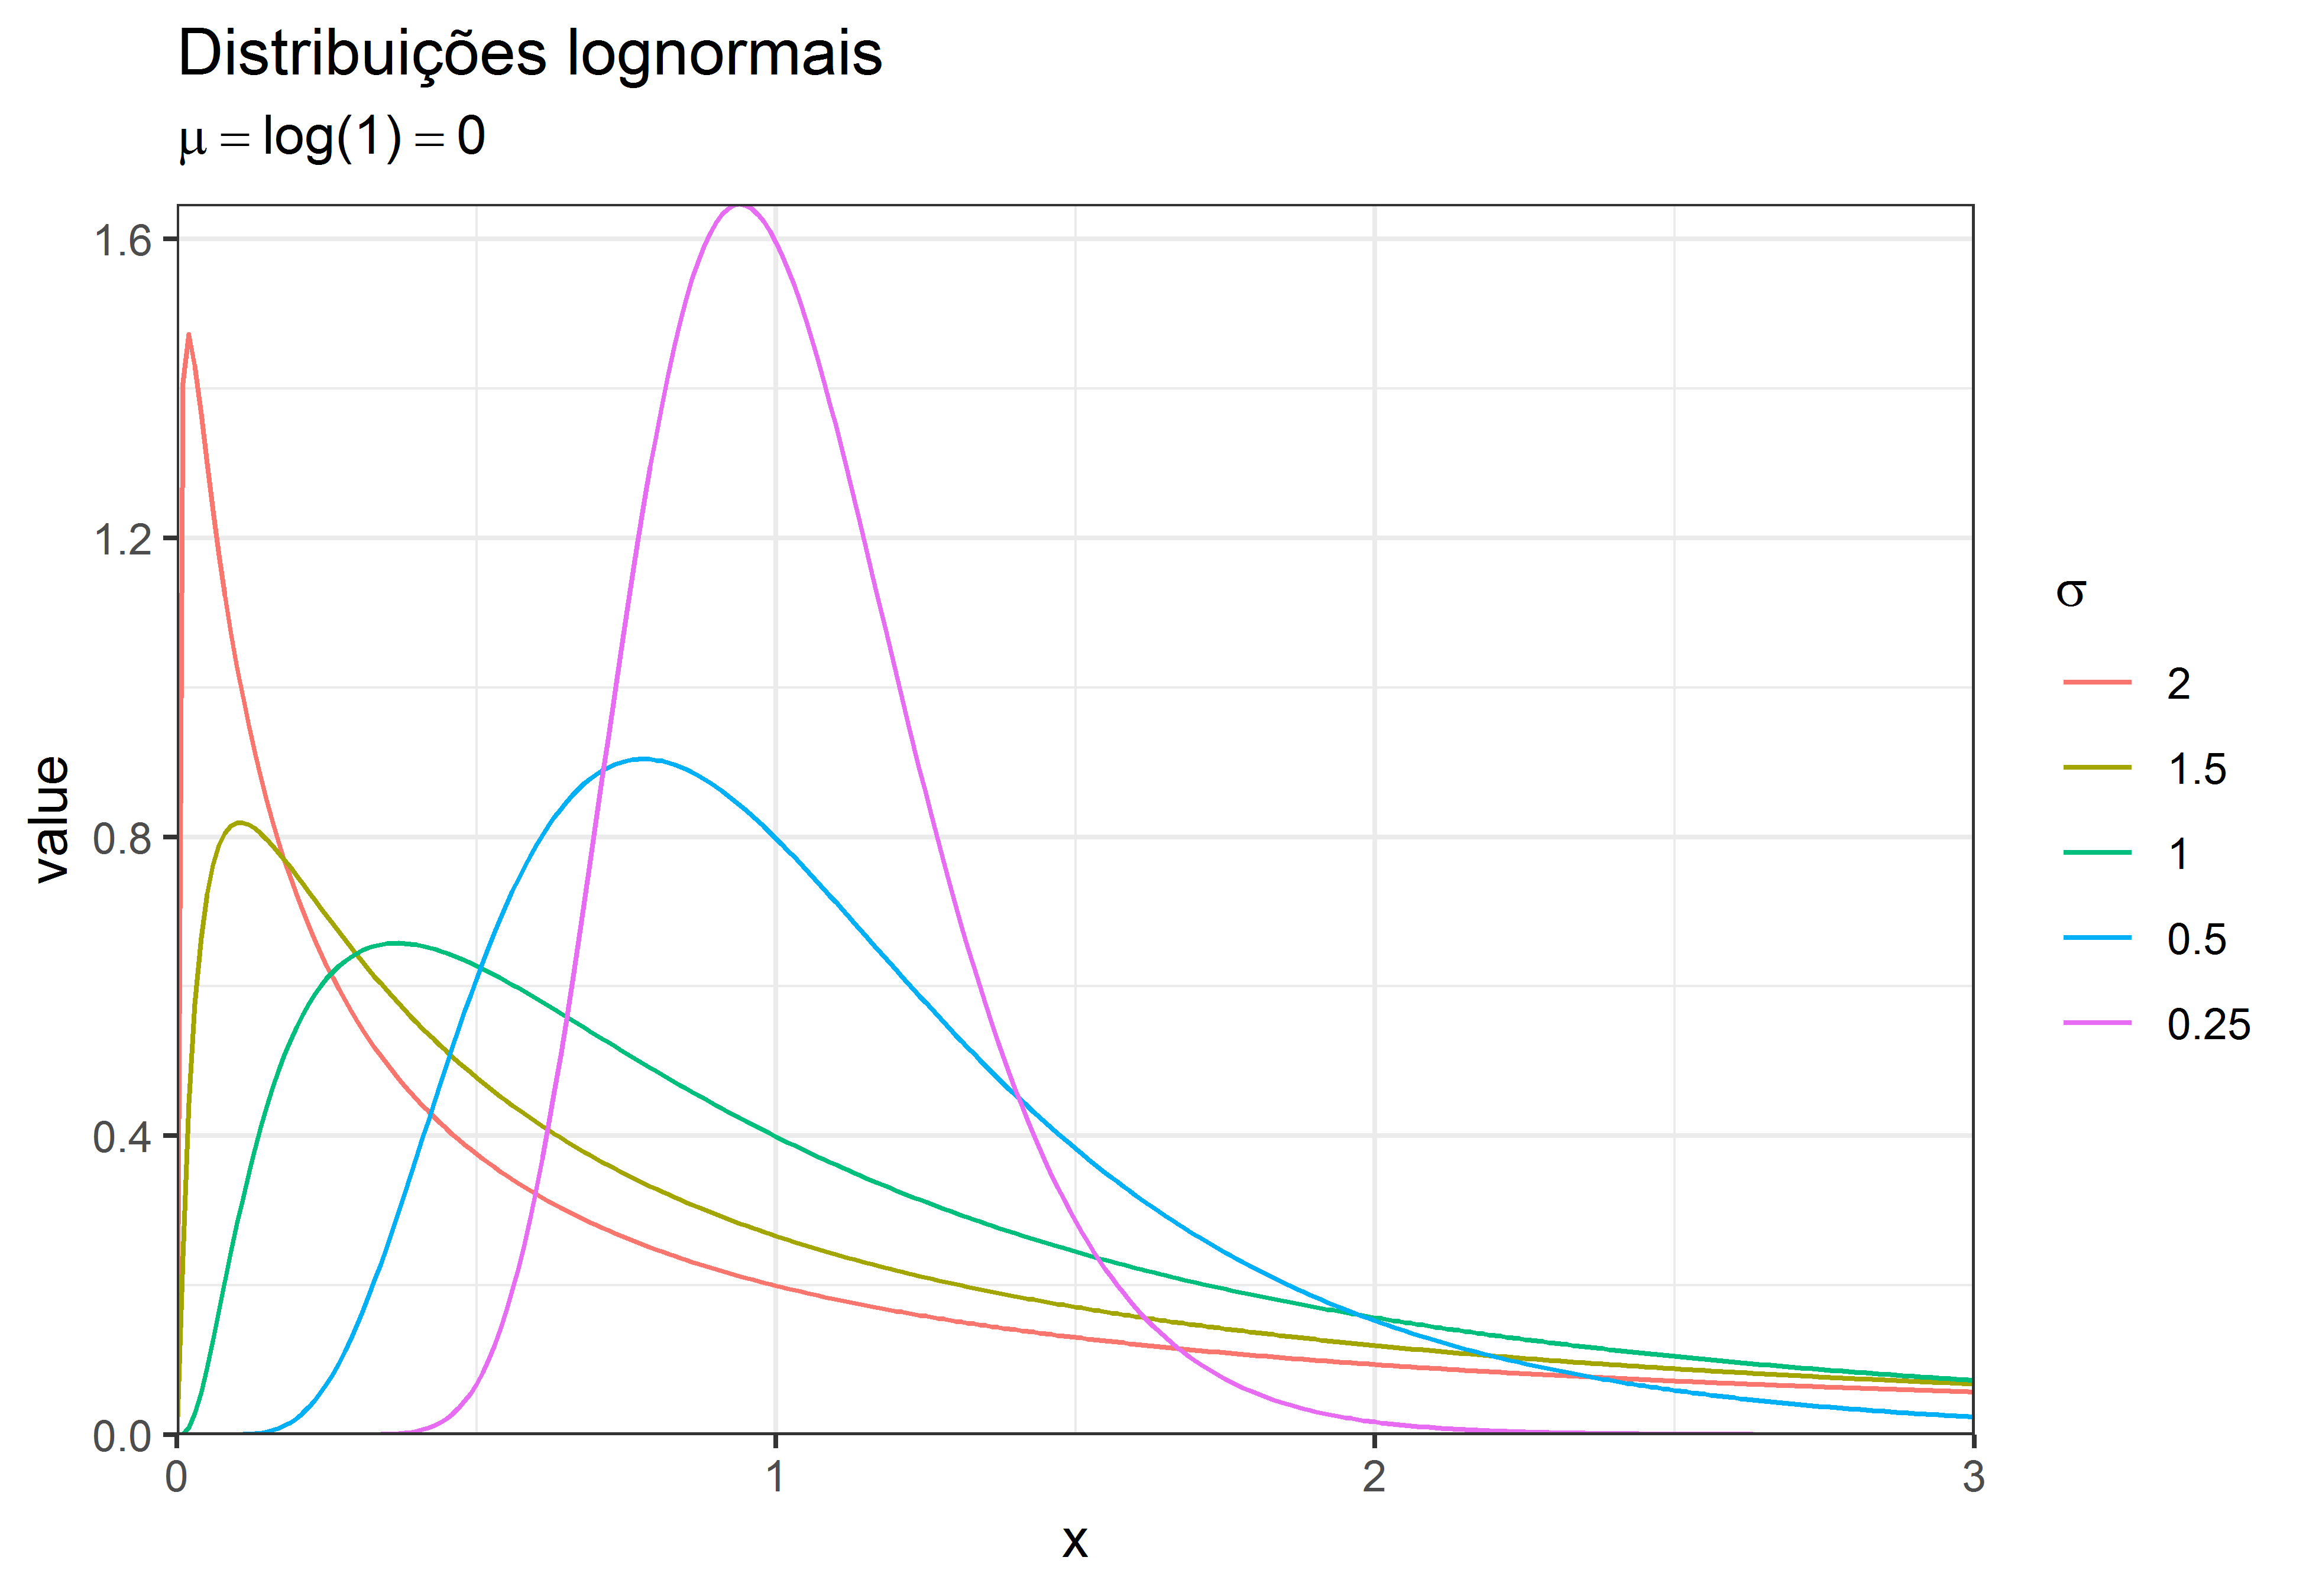
\includegraphics[width=0.5\linewidth]{images/logs-1} 

}

\caption{Distribuição lognormal com $\mu = 0$ e diversos valores de $\sigma$}\label{fig:logs}
\end{figure}

\begin{center}\animategraphics[width=0.5\linewidth,controls,loop]{10}{images/video-}{1}{14}\end{center}

\subsubsection{Relação com a distribuição
normal}\label{relacao-com-a-distribuicao-normal}

Lembrando que a função densidade de probabilidade de uma variável
aleatória com distribuição normal é dada por:

\[f(t) = \frac{1}{\sigma\sqrt{2\pi}}\mathrm{e}^{-\frac{1}{2}\frac{(t-\mu)^2}{\sigma^2}}\]
E que para a distribuição normal-padrão (\(N(0,1)\)) a função densidade
de probabilidade torna-se:

\[\varphi(t) = \frac{1}{\sqrt{2\pi}}\mathrm{e}^{-\frac{1}{2}t^2}\]

Seja \(X\) uma variável aleatória de distribuição normal padronizada
(\(X \sim N(0, 1)\)), \(f_X\) a função densidade de probabilidade e
\(Y = e^X\). Então (\(F_Y\)) é igual a:

\[F_Y(y) = \mathbb{P}(e^X\leq y) = \mathbb{P}(X \leq ln(Y)) = \int_{-\infty}^{ln(y)}f_X(x)dx = \int_{-\infty}^{ln(y)}\frac{1}{\sqrt{2\pi}}e^{-x^2/2}dx\]
o que equivale a:

\[F_Y(y) = \int_{0}^{y}\frac{1}{x}\frac{1}{\sqrt{2\pi}}e^{-ln(x)^2/2}\]

Ou seja, a distribuição de uma variável \(Y = e^X\), em que
\(X \sim N(0,1)\) é equivalente a distribuição de uma variável lognormal
com parâmetros \(\mu = 0\) e \(\sigma = 1\).

A figura \ref{fig:normal_lognormal} ilustra este fato.

\begin{figure}[H]

{\centering 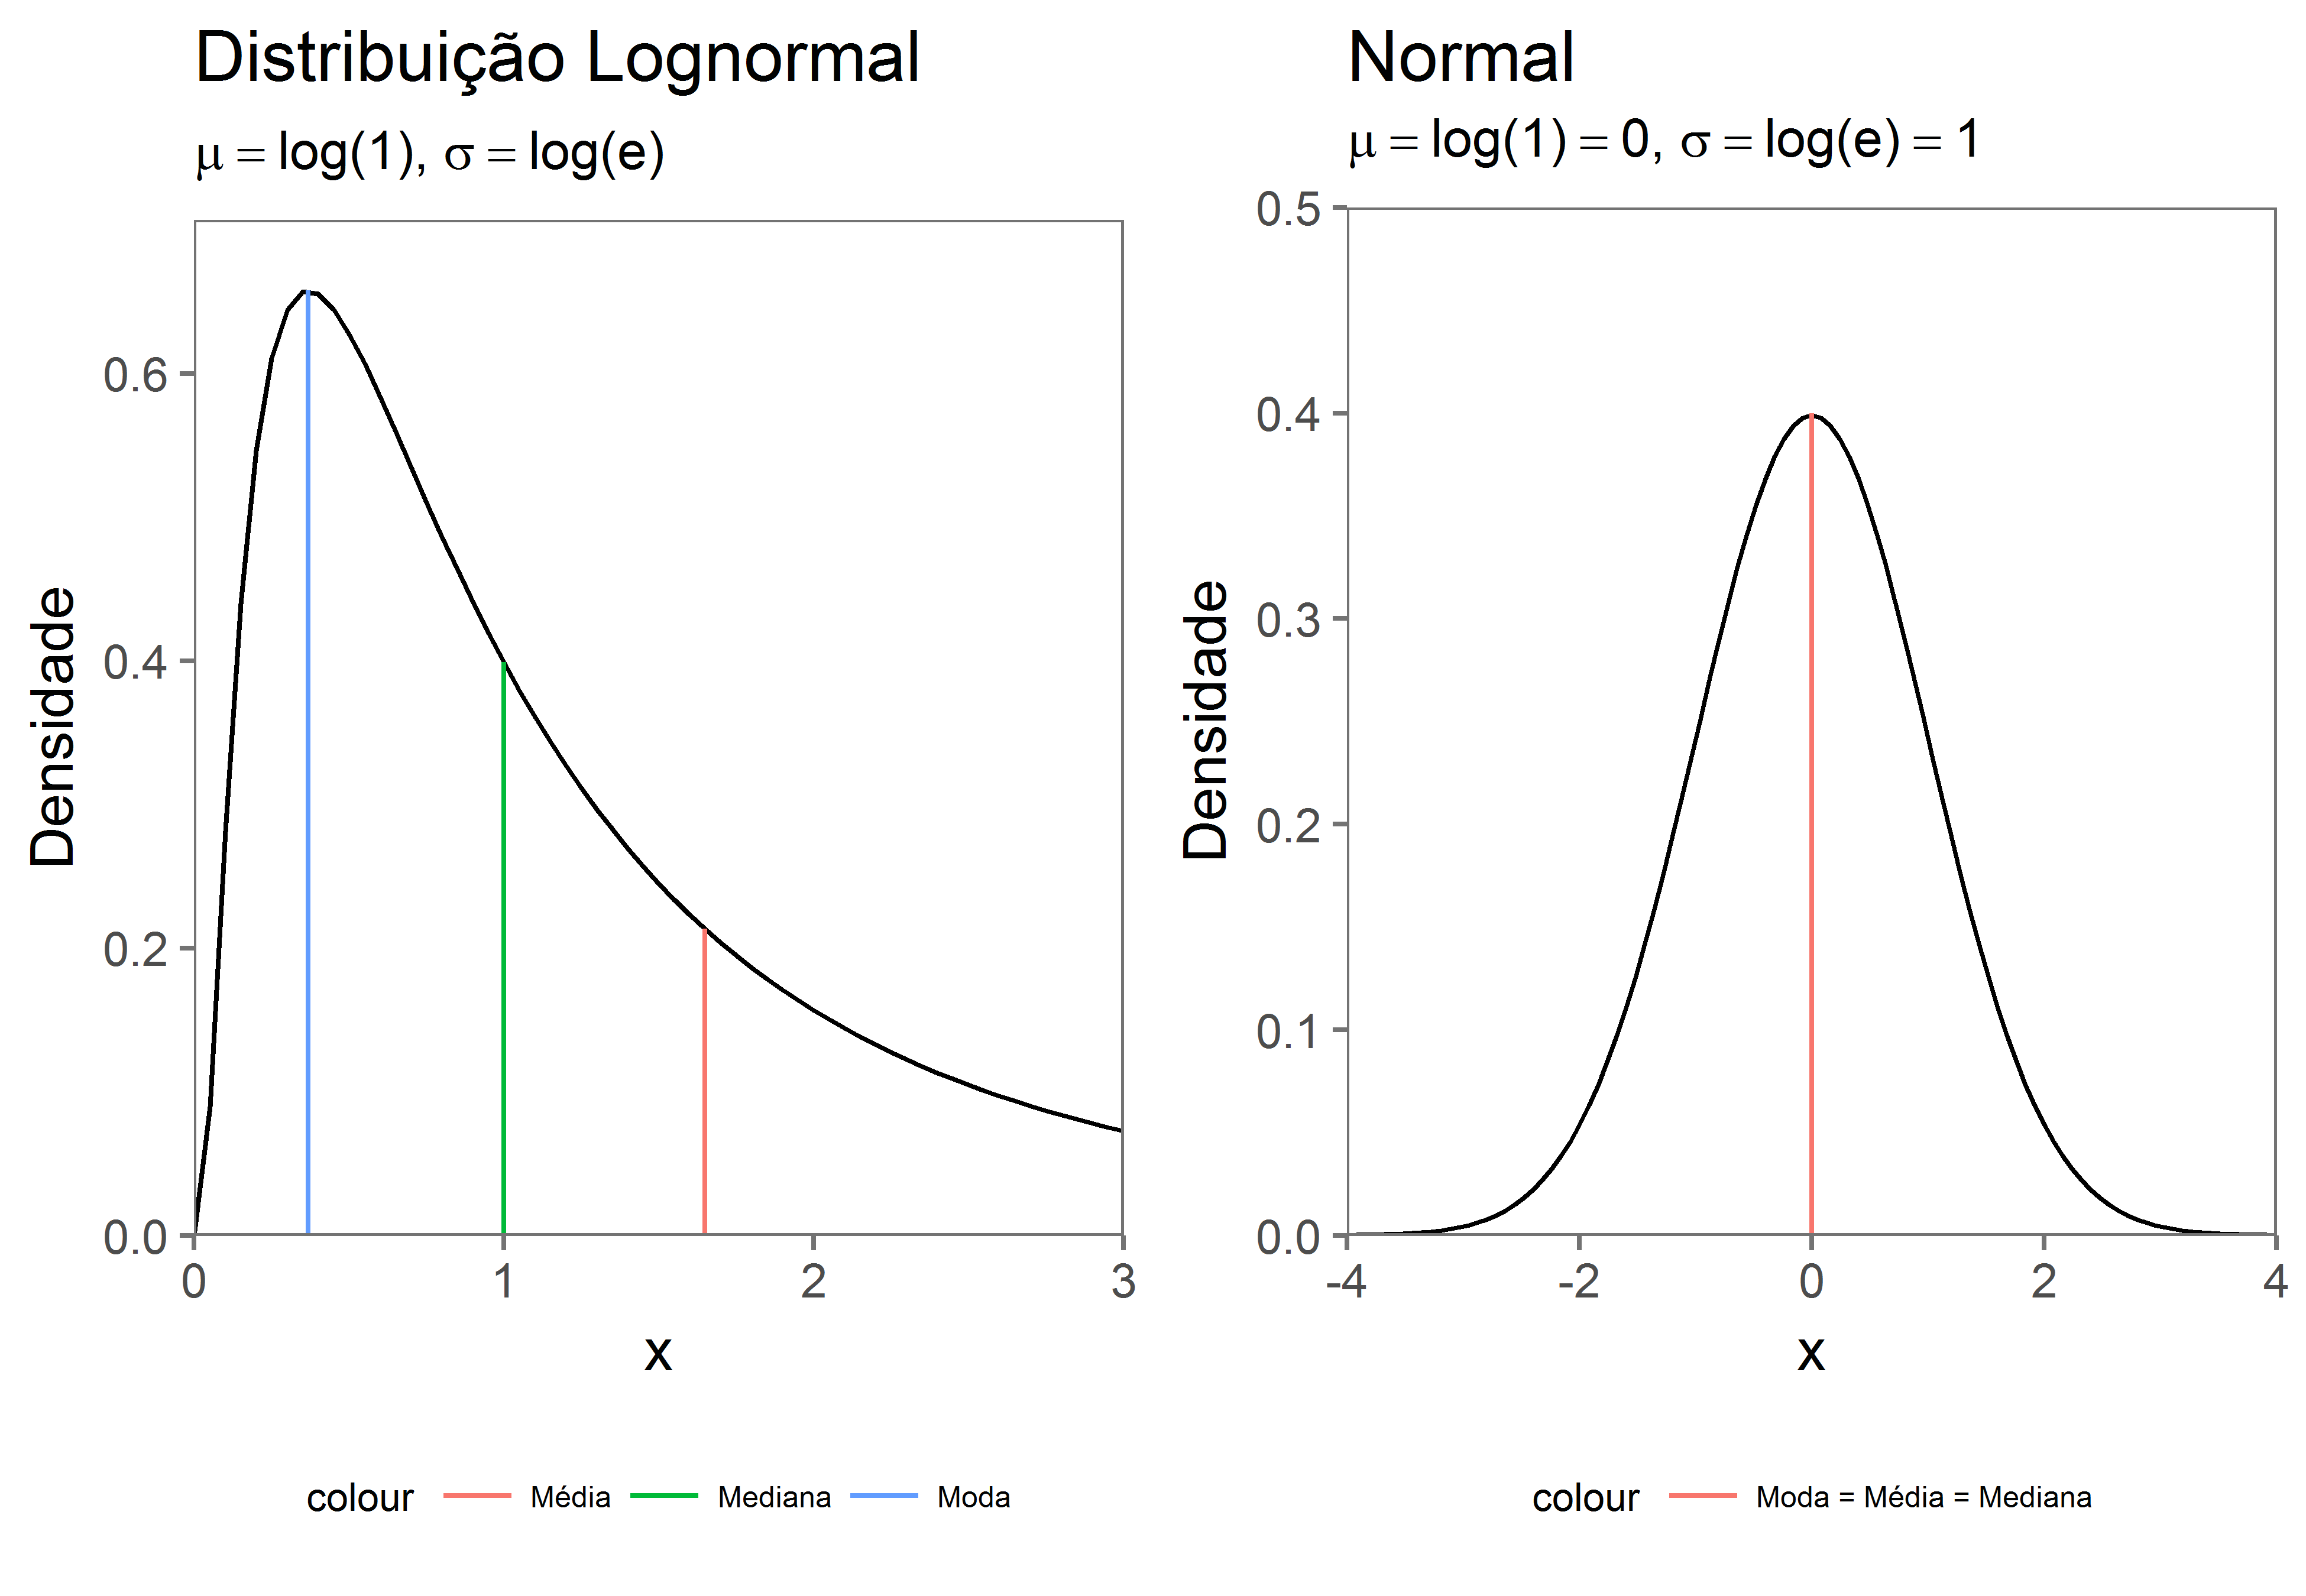
\includegraphics[width=1\linewidth]{images/normal_lognormal-1} 

}

\caption{Comparação entre distribuições normal e lognormal padronizadas.}\label{fig:normal_lognormal}
\end{figure}

\subsubsection{Analogia com o Teorema do Limite
Central}\label{analogia-com-o-teorema-do-limite-central}

Assim como o resultado da soma de diversas variáveis independentes com
distribuições quaisquer resulta numa variável aleatória de distribuição
normal (Teorema do Limite Central), o produto de diversas variáveis
aleatórias resulta numa distribuição lognormal.

\subsubsection{Transformação de variável e
Homoscedasticidade}\label{transformacao-de-variavel-e-homoscedasticidade}

De acordo com Matloff (\protect\hyperlink{ref-matloff2017}{2017}, p.
138), se uma variável aleatória \(W\) é aproximadamente normal, com
baixo coeficiente de variação (\(CV = \sigma/\mu\)), e \(g(W)\) é uma
função suave, então a nova variável também será aproximadamente normal,
com média \(g(EW)\) e variância:

\[[g'(EW)]^2\text{Var}(W)\]

Assumindo que os erros de uma função de regressão sejam
heteroscedásticos, seguindo uma função conhecida \(\sigma(t) = \mu(t)\),
se aplicarmos a função logaritmo natural à variável dependente, segundo
a equação acima, teremos\footnote{Lembrando que a derivada da função
  logaritmo natural é \(\frac{d}{dt}\ln t= \frac{1}{t}\) e que
  \(\text{Var}(W) = \sigma^2(W)\)}:

\[\frac{1}{\mu^2(t)}\mu^2(t) = 1\]

Ou seja, o uso da transformação logaritmo natural, para este caso em
particular, conduz à homoscedasticidade do modelo.

De acordo com Matloff (\protect\hyperlink{ref-matloff2017}{2017}, p.
138), ainda, se \(\sigma(t) = \sqrt{\mu(t)}\), a transformação
raiz-quadrada é que traria de volta a homoscedasticidade.\footnote{\(\frac{d}{dt}\sqrt{t} = \frac{0,5}{\sqrt{t}} \rightarrow \text{Var}(\sqrt{W}) = \left (\frac{0,5}{\sqrt{t}} \right)^2(\sqrt{t})^2 = 0,25\)}

\section{EXEMPLO}\label{exemplo}

\subsection{Dados}\label{dados}

Os dados utilizados aqui são oriundos de Hochheim
(\protect\hyperlink{ref-hochheim}{2015}, pp. 21--22) e são reproduzidos
no \protect\hyperlink{anexo-i}{ANEXO I}.

\subsection{Ajuste de distribuições aos
dados}\label{ajuste-de-distribuicoes-aos-dados}

\begin{figure}[H]

{\centering 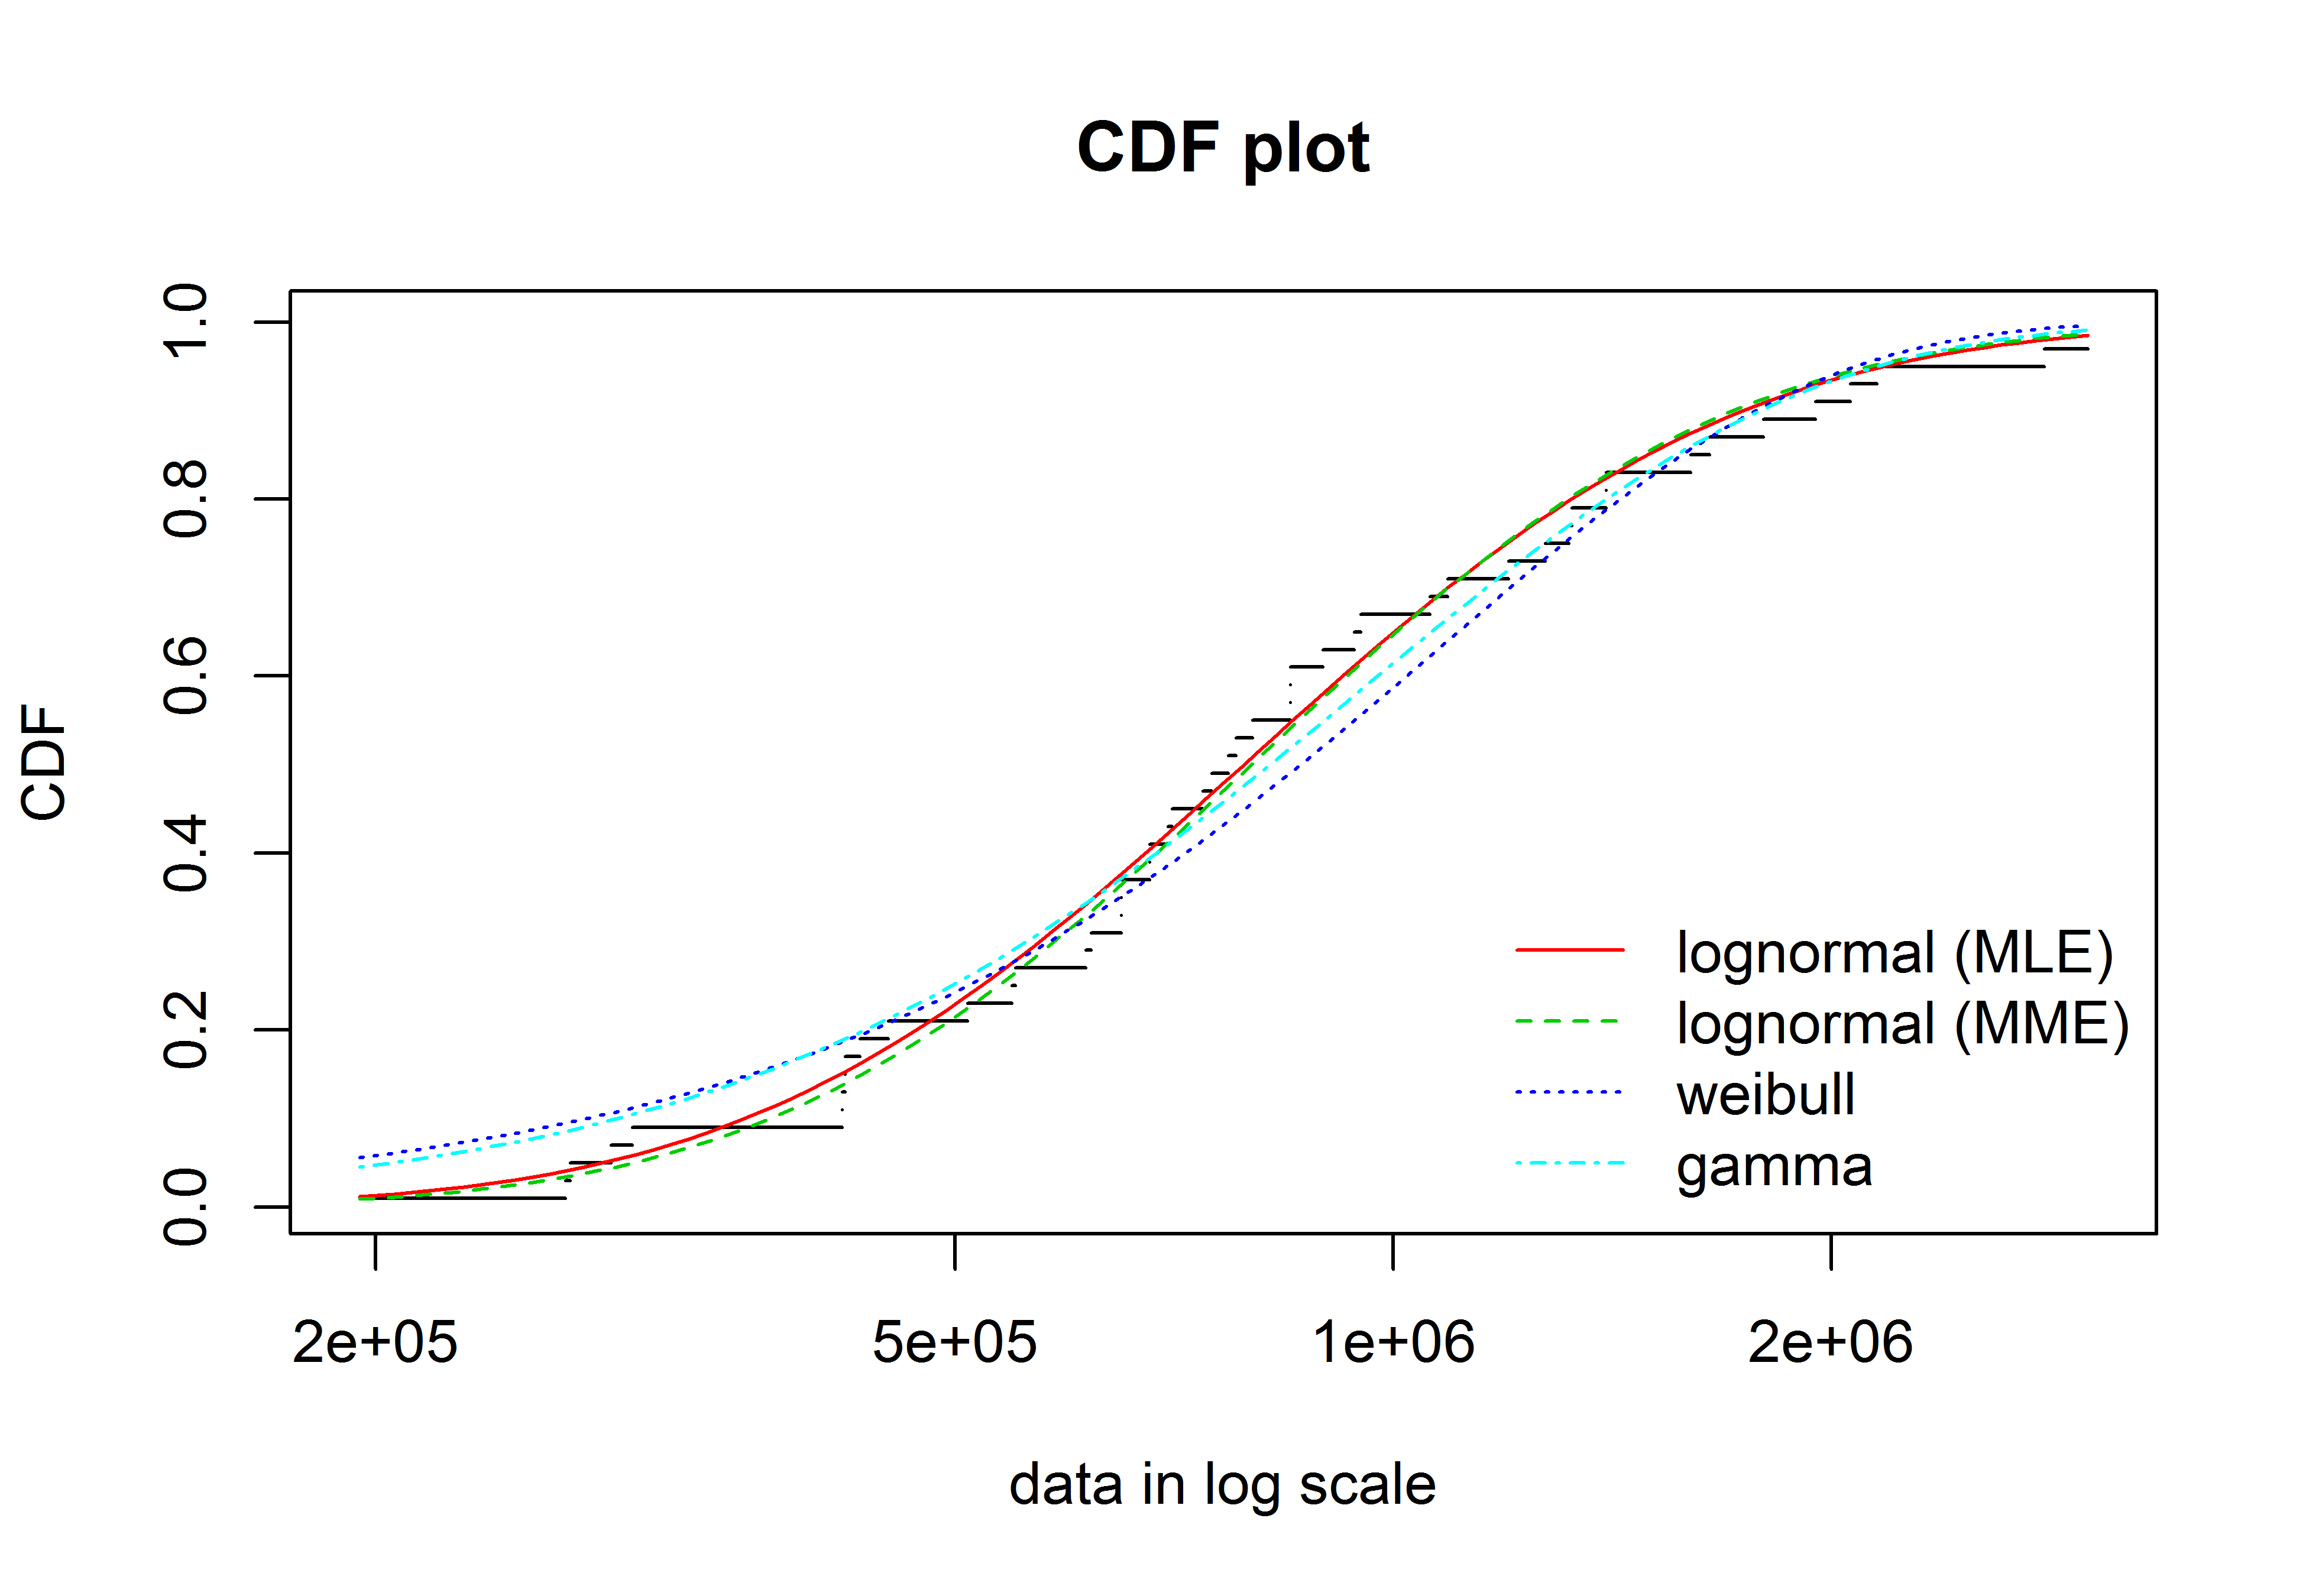
\includegraphics[width=0.49\linewidth]{images/fitdist-1} 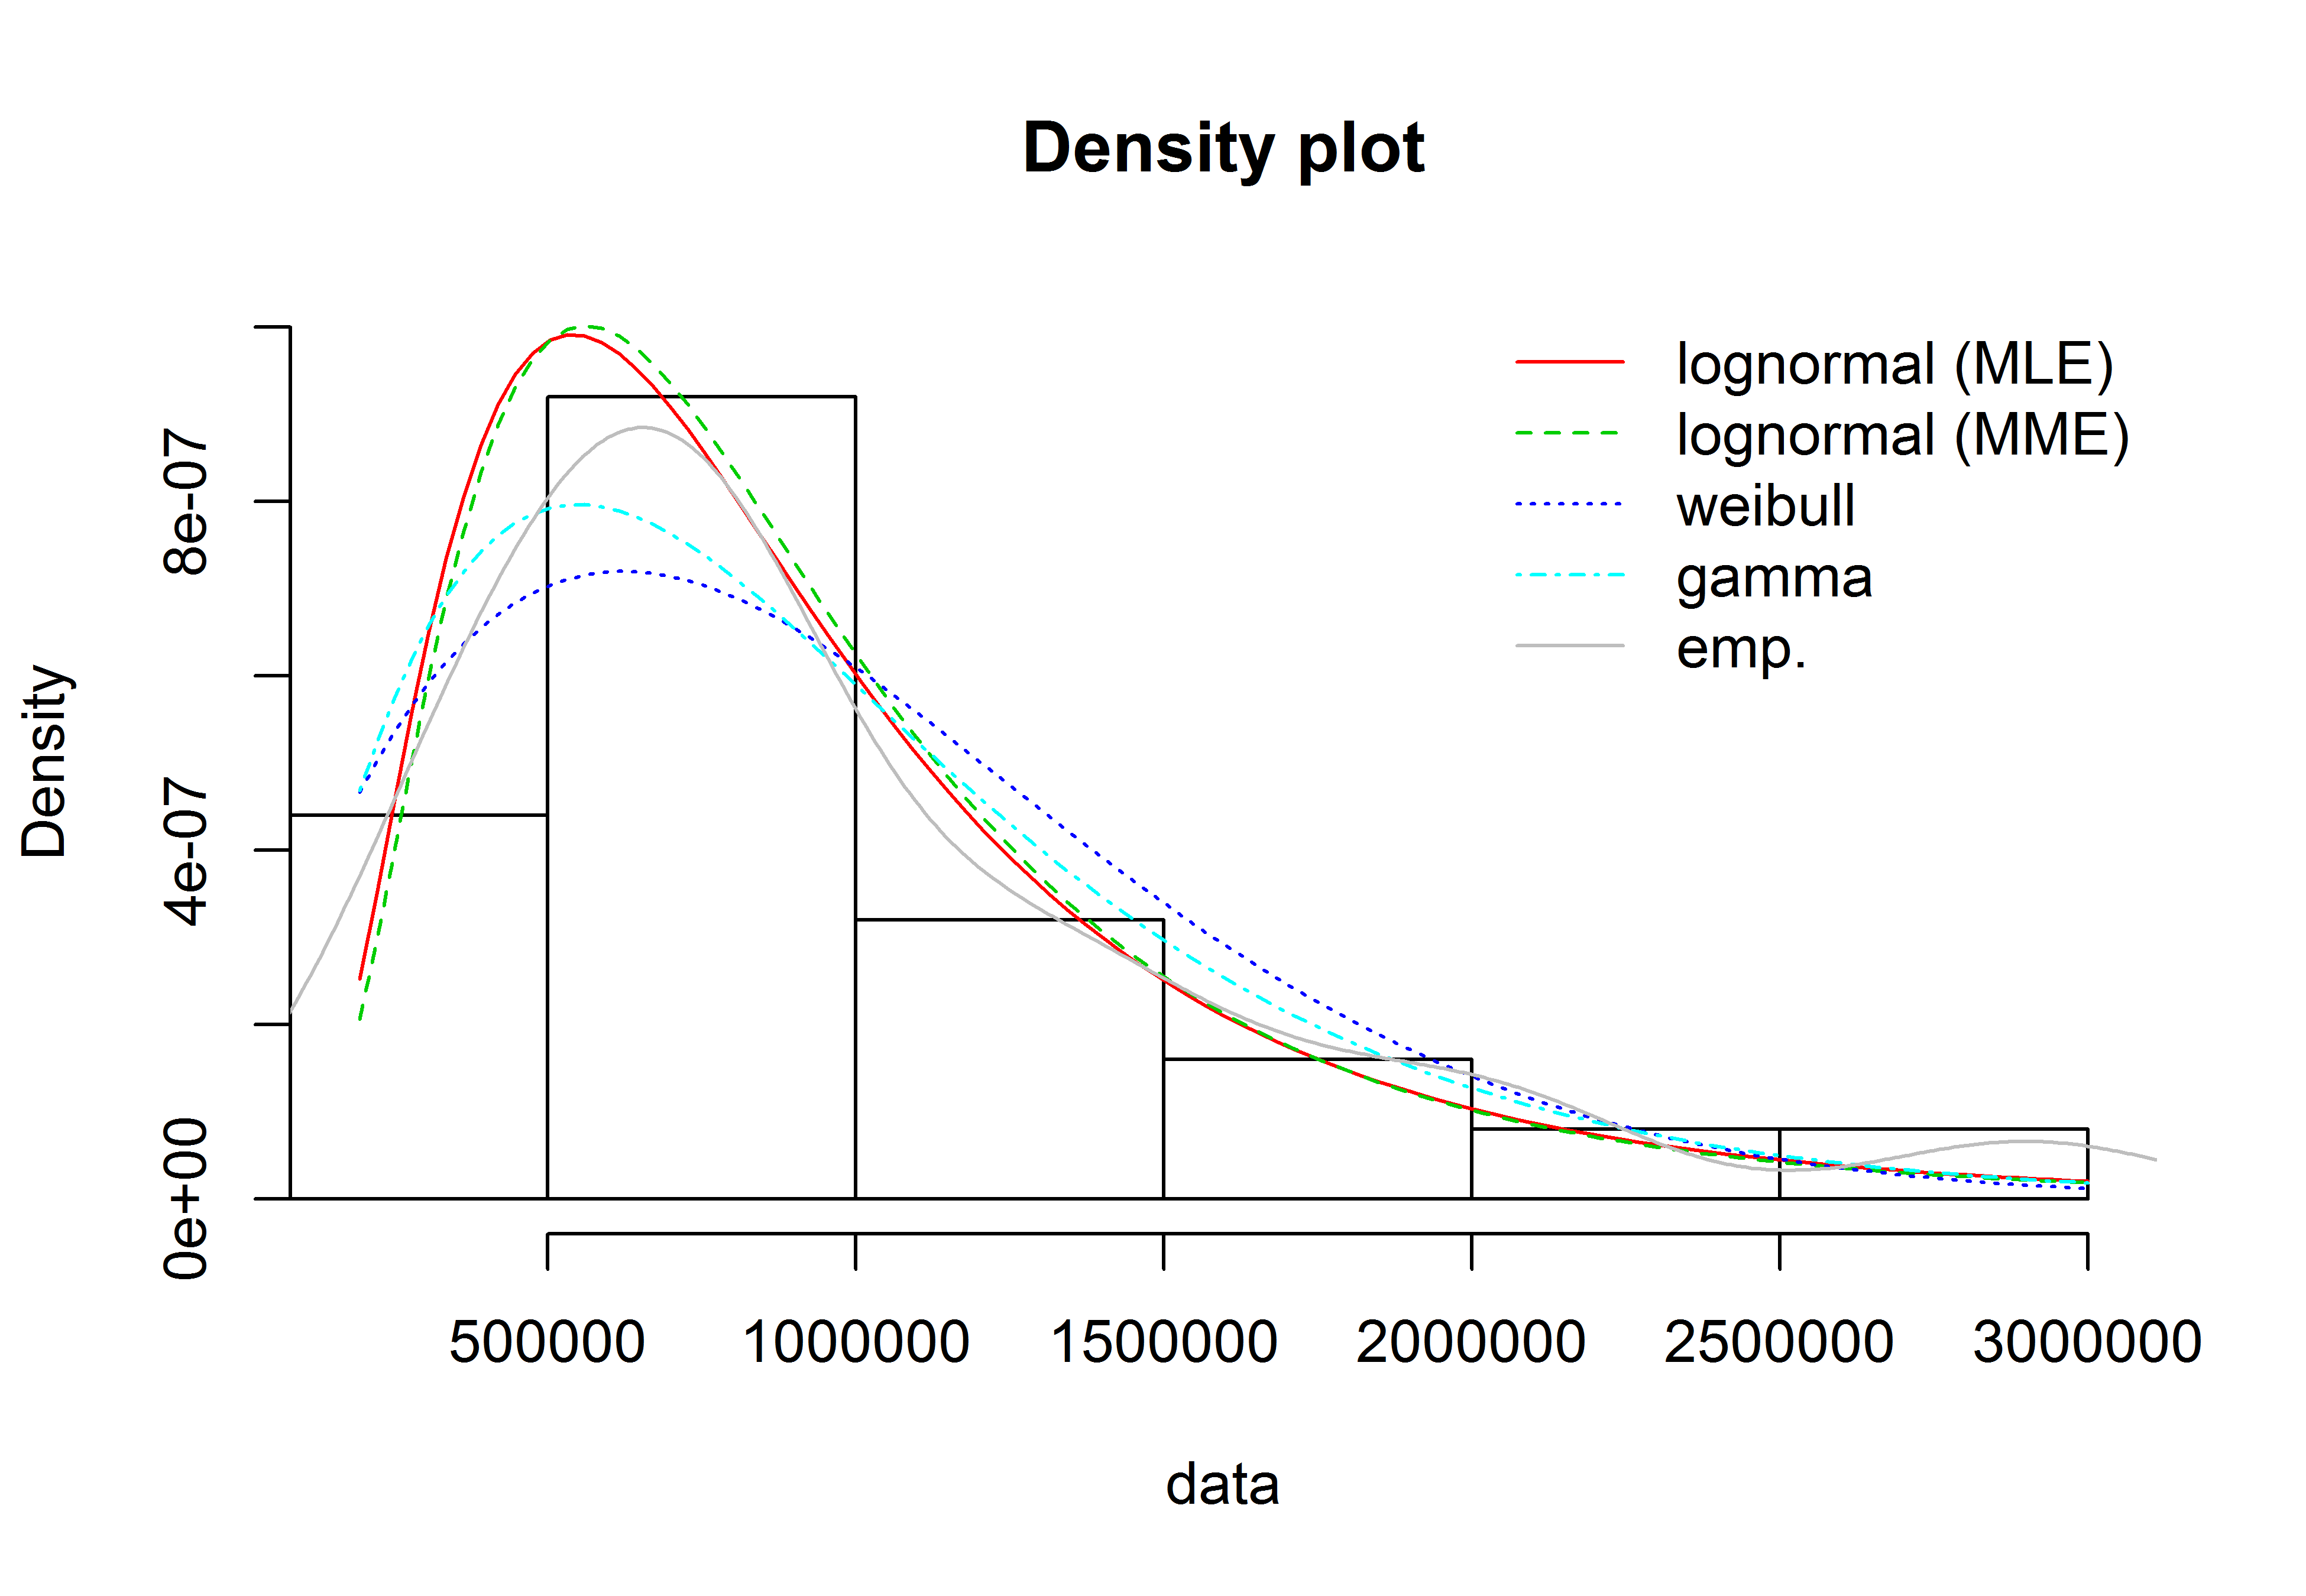
\includegraphics[width=0.49\linewidth]{images/fitdist-2} 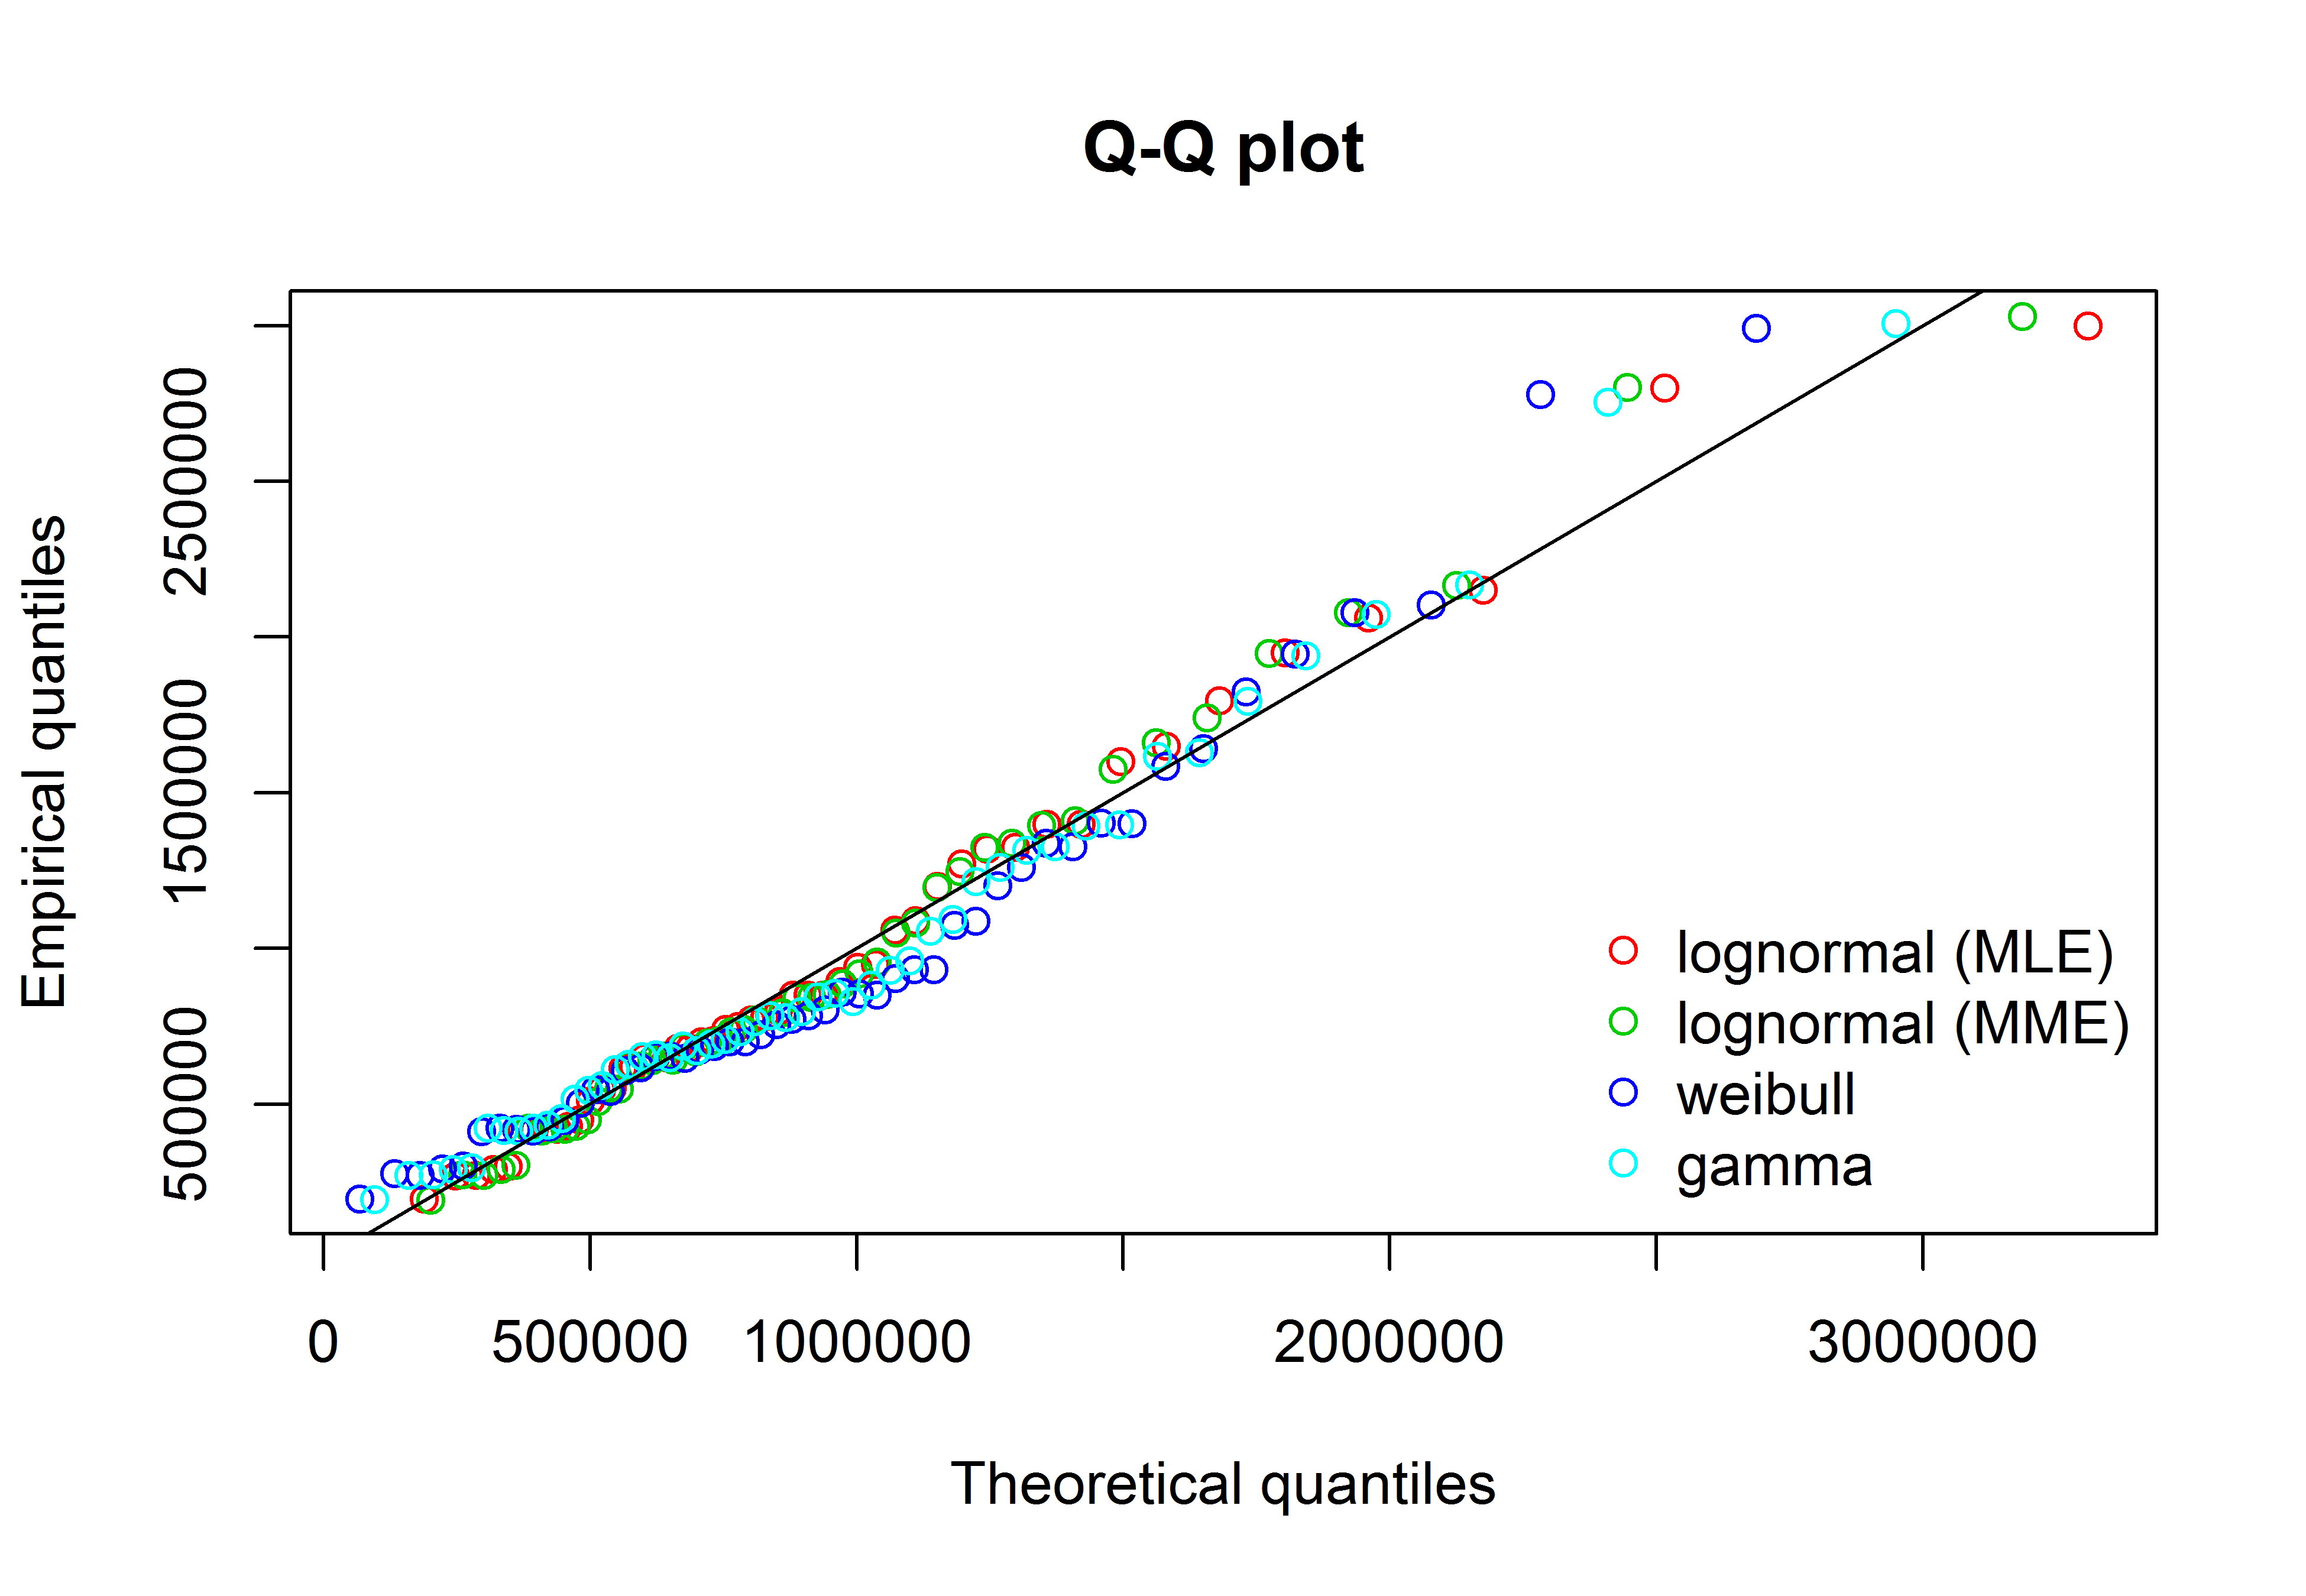
\includegraphics[width=0.49\linewidth]{images/fitdist-3} 

}

\caption{Ajuste da distribuição empírica a diversas distribuições teóricas.}\label{fig:fitdist}
\end{figure}

Percebe-se pela análise das figuras \ref{fig:fitdist} que o melhor
ajuste se deu para a distribuição lognormal ajustada seja pelo método
dos momentos (MME) ou pelo método da verossimilhança (MLE), haja vista
que as outras distribuições inicialmente crescem mais rapidamente e tem
pico mais achatado que os dados empíricos e as distribuições log-normais
ajustadas.

\subsection{Gráficos}\label{graficos}

As figuras \ref{fig:densidade} a \ref{fig:hist_densidade2} mostram que
os valores observados para a variável \code{valor} do conjunto de dados
mencionados acima (HOCHHEIM, \protect\hyperlink{ref-hochheim}{2015}, pp.
21--22) apresentam distribuição aproximadamente lognormal, com
parâmetros \(\mu = \bar{ln(valor)}\)

\newpage

\begin{enumerate}
\def\labelenumi{\alph{enumi}.}
\tightlist
\item
  Densidade
\end{enumerate}

A figura \ref{fig:densidade} mostra o gráfico da função densidade de
probabilidade (FDP) construídos com os parâmetros \(\mu\) e \(\sigma\)
obtidos da variável valor.

\begin{figure}[H]

{\centering 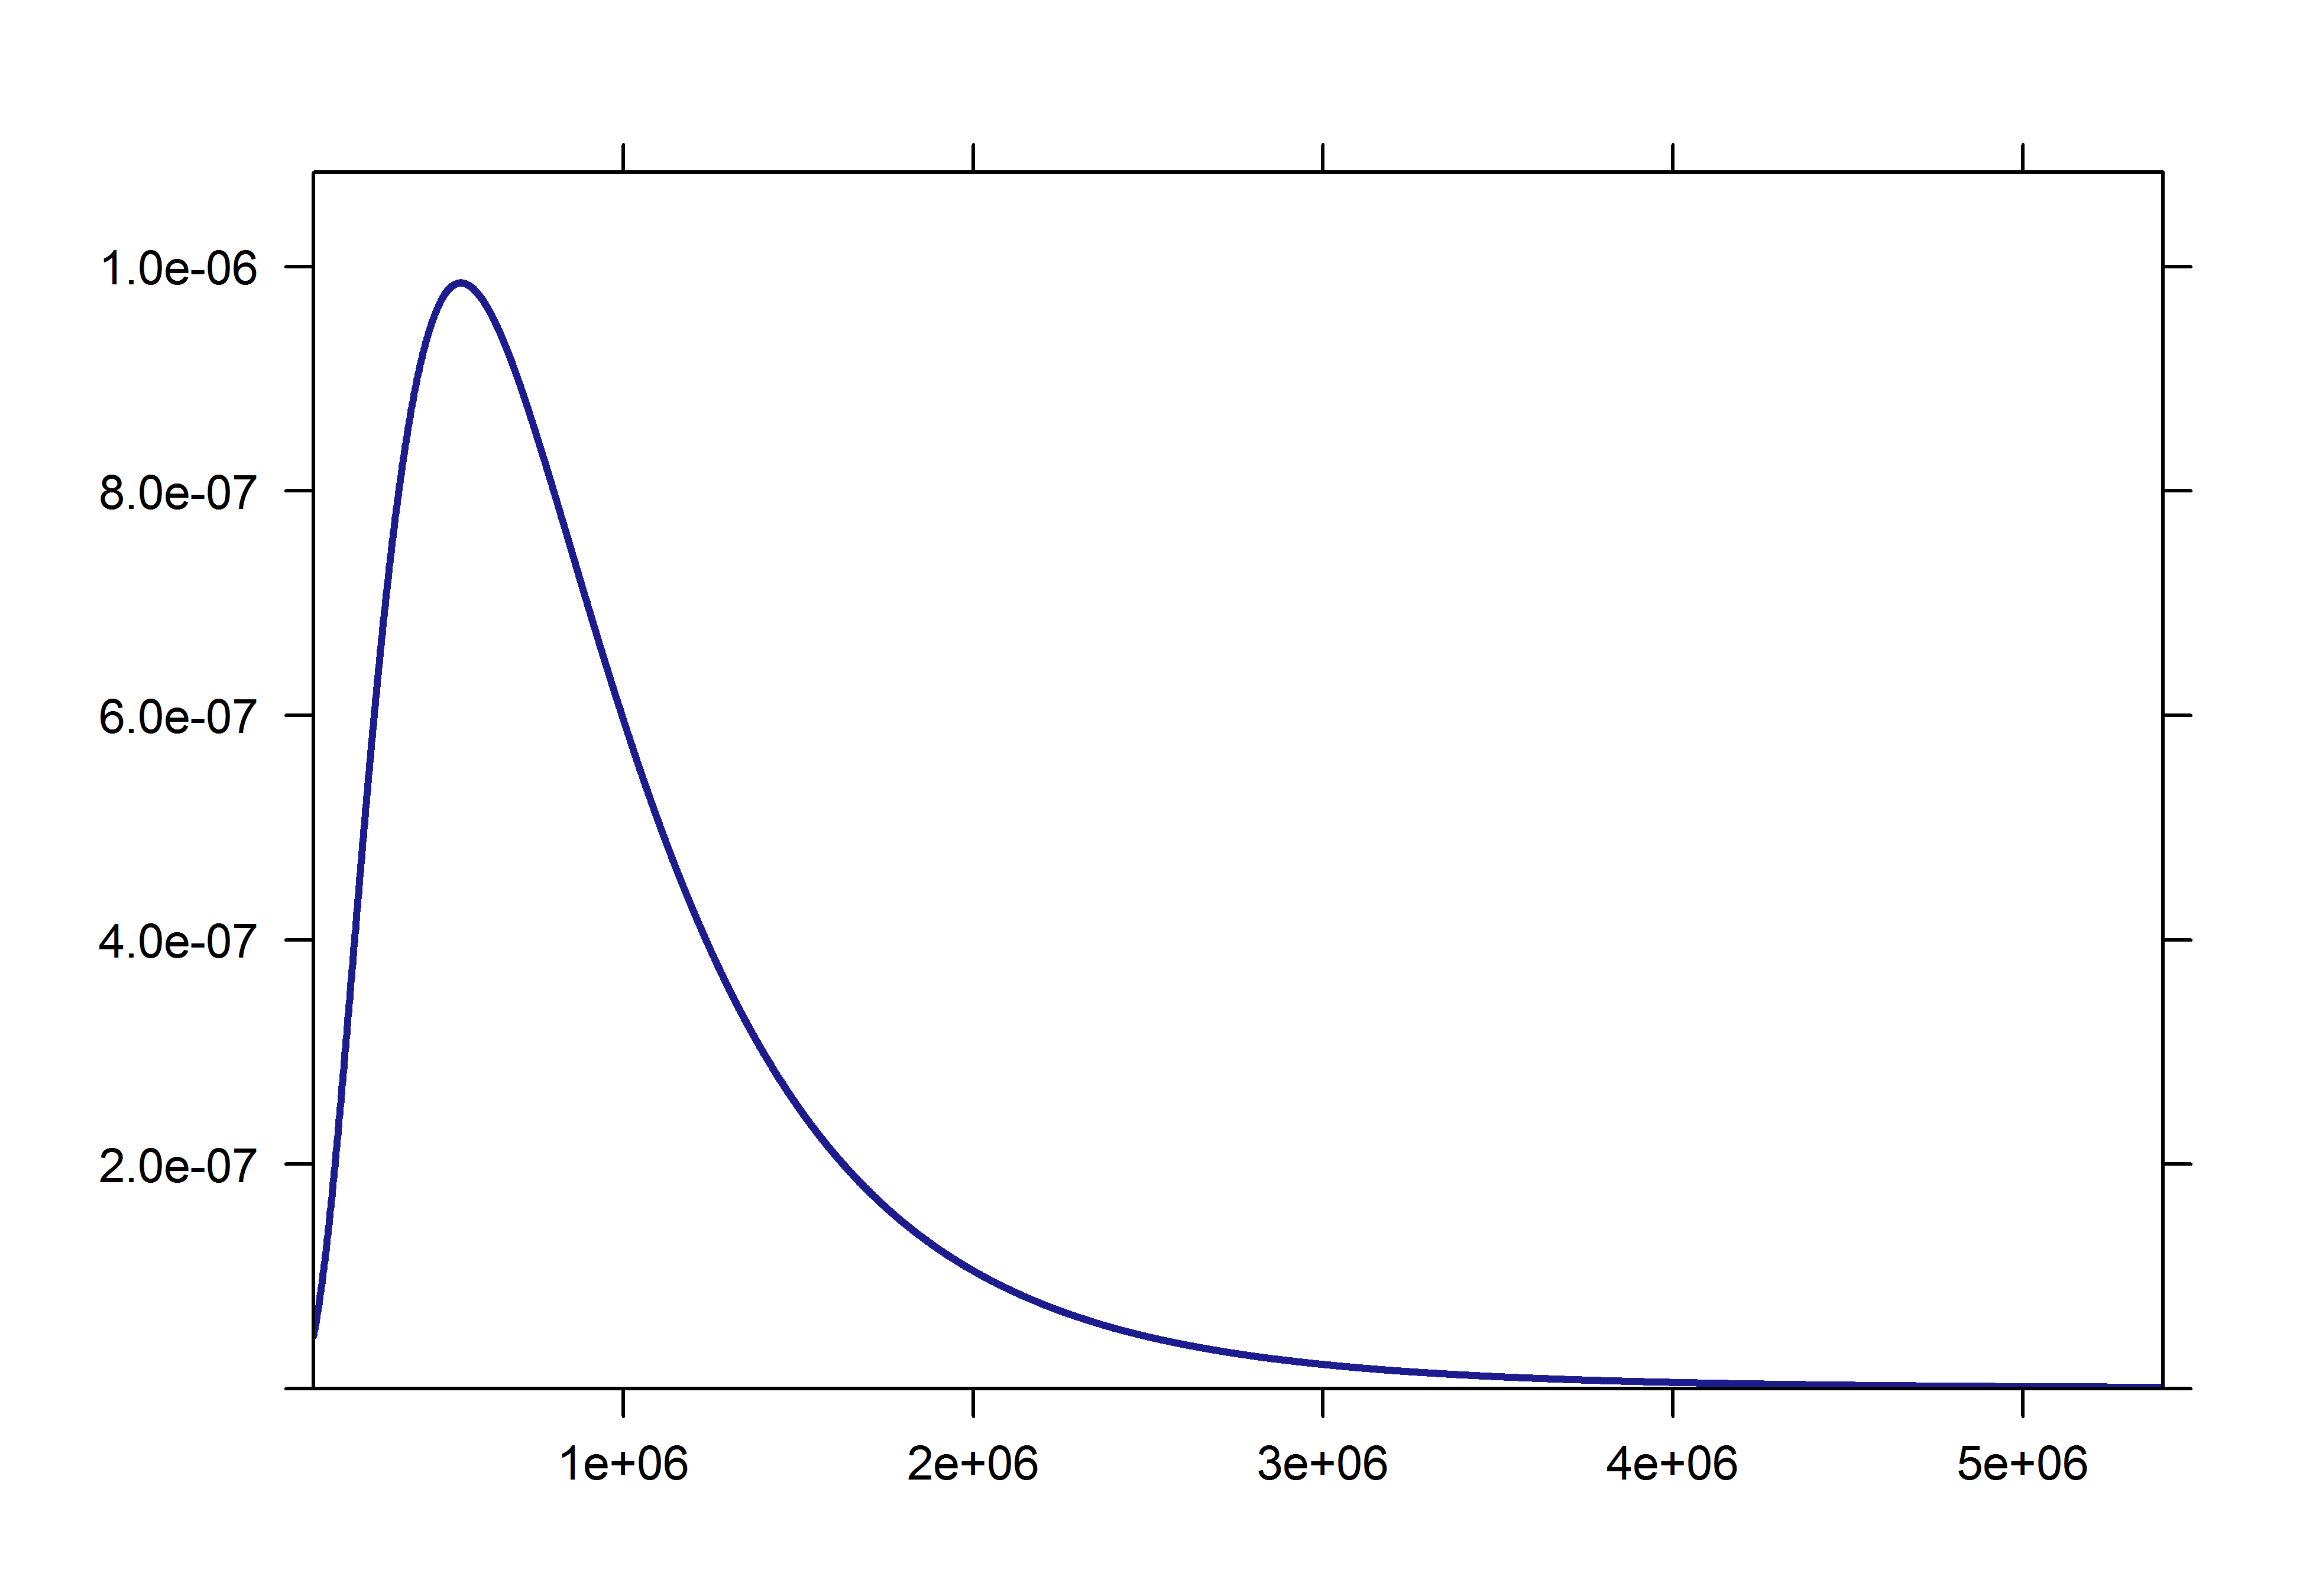
\includegraphics[width=0.5\linewidth]{images/densidade-1} 

}

\caption{Função densidade de probabilidade com parâmetros obtidos dos dados da variável \code{valor}}\label{fig:densidade}
\end{figure}

\begin{enumerate}
\def\labelenumi{\alph{enumi}.}
\setcounter{enumi}{1}
\tightlist
\item
  Histograma com densidade superposta
\end{enumerate}

A figura \ref{fig:hist_densidade} mostra o histograma dos dados da
variável \texttt{valor}, superposto com a curva da função densidade de
probabilidade (FDP) da figura \ref{fig:densidade}.

\begin{figure}[H]

{\centering 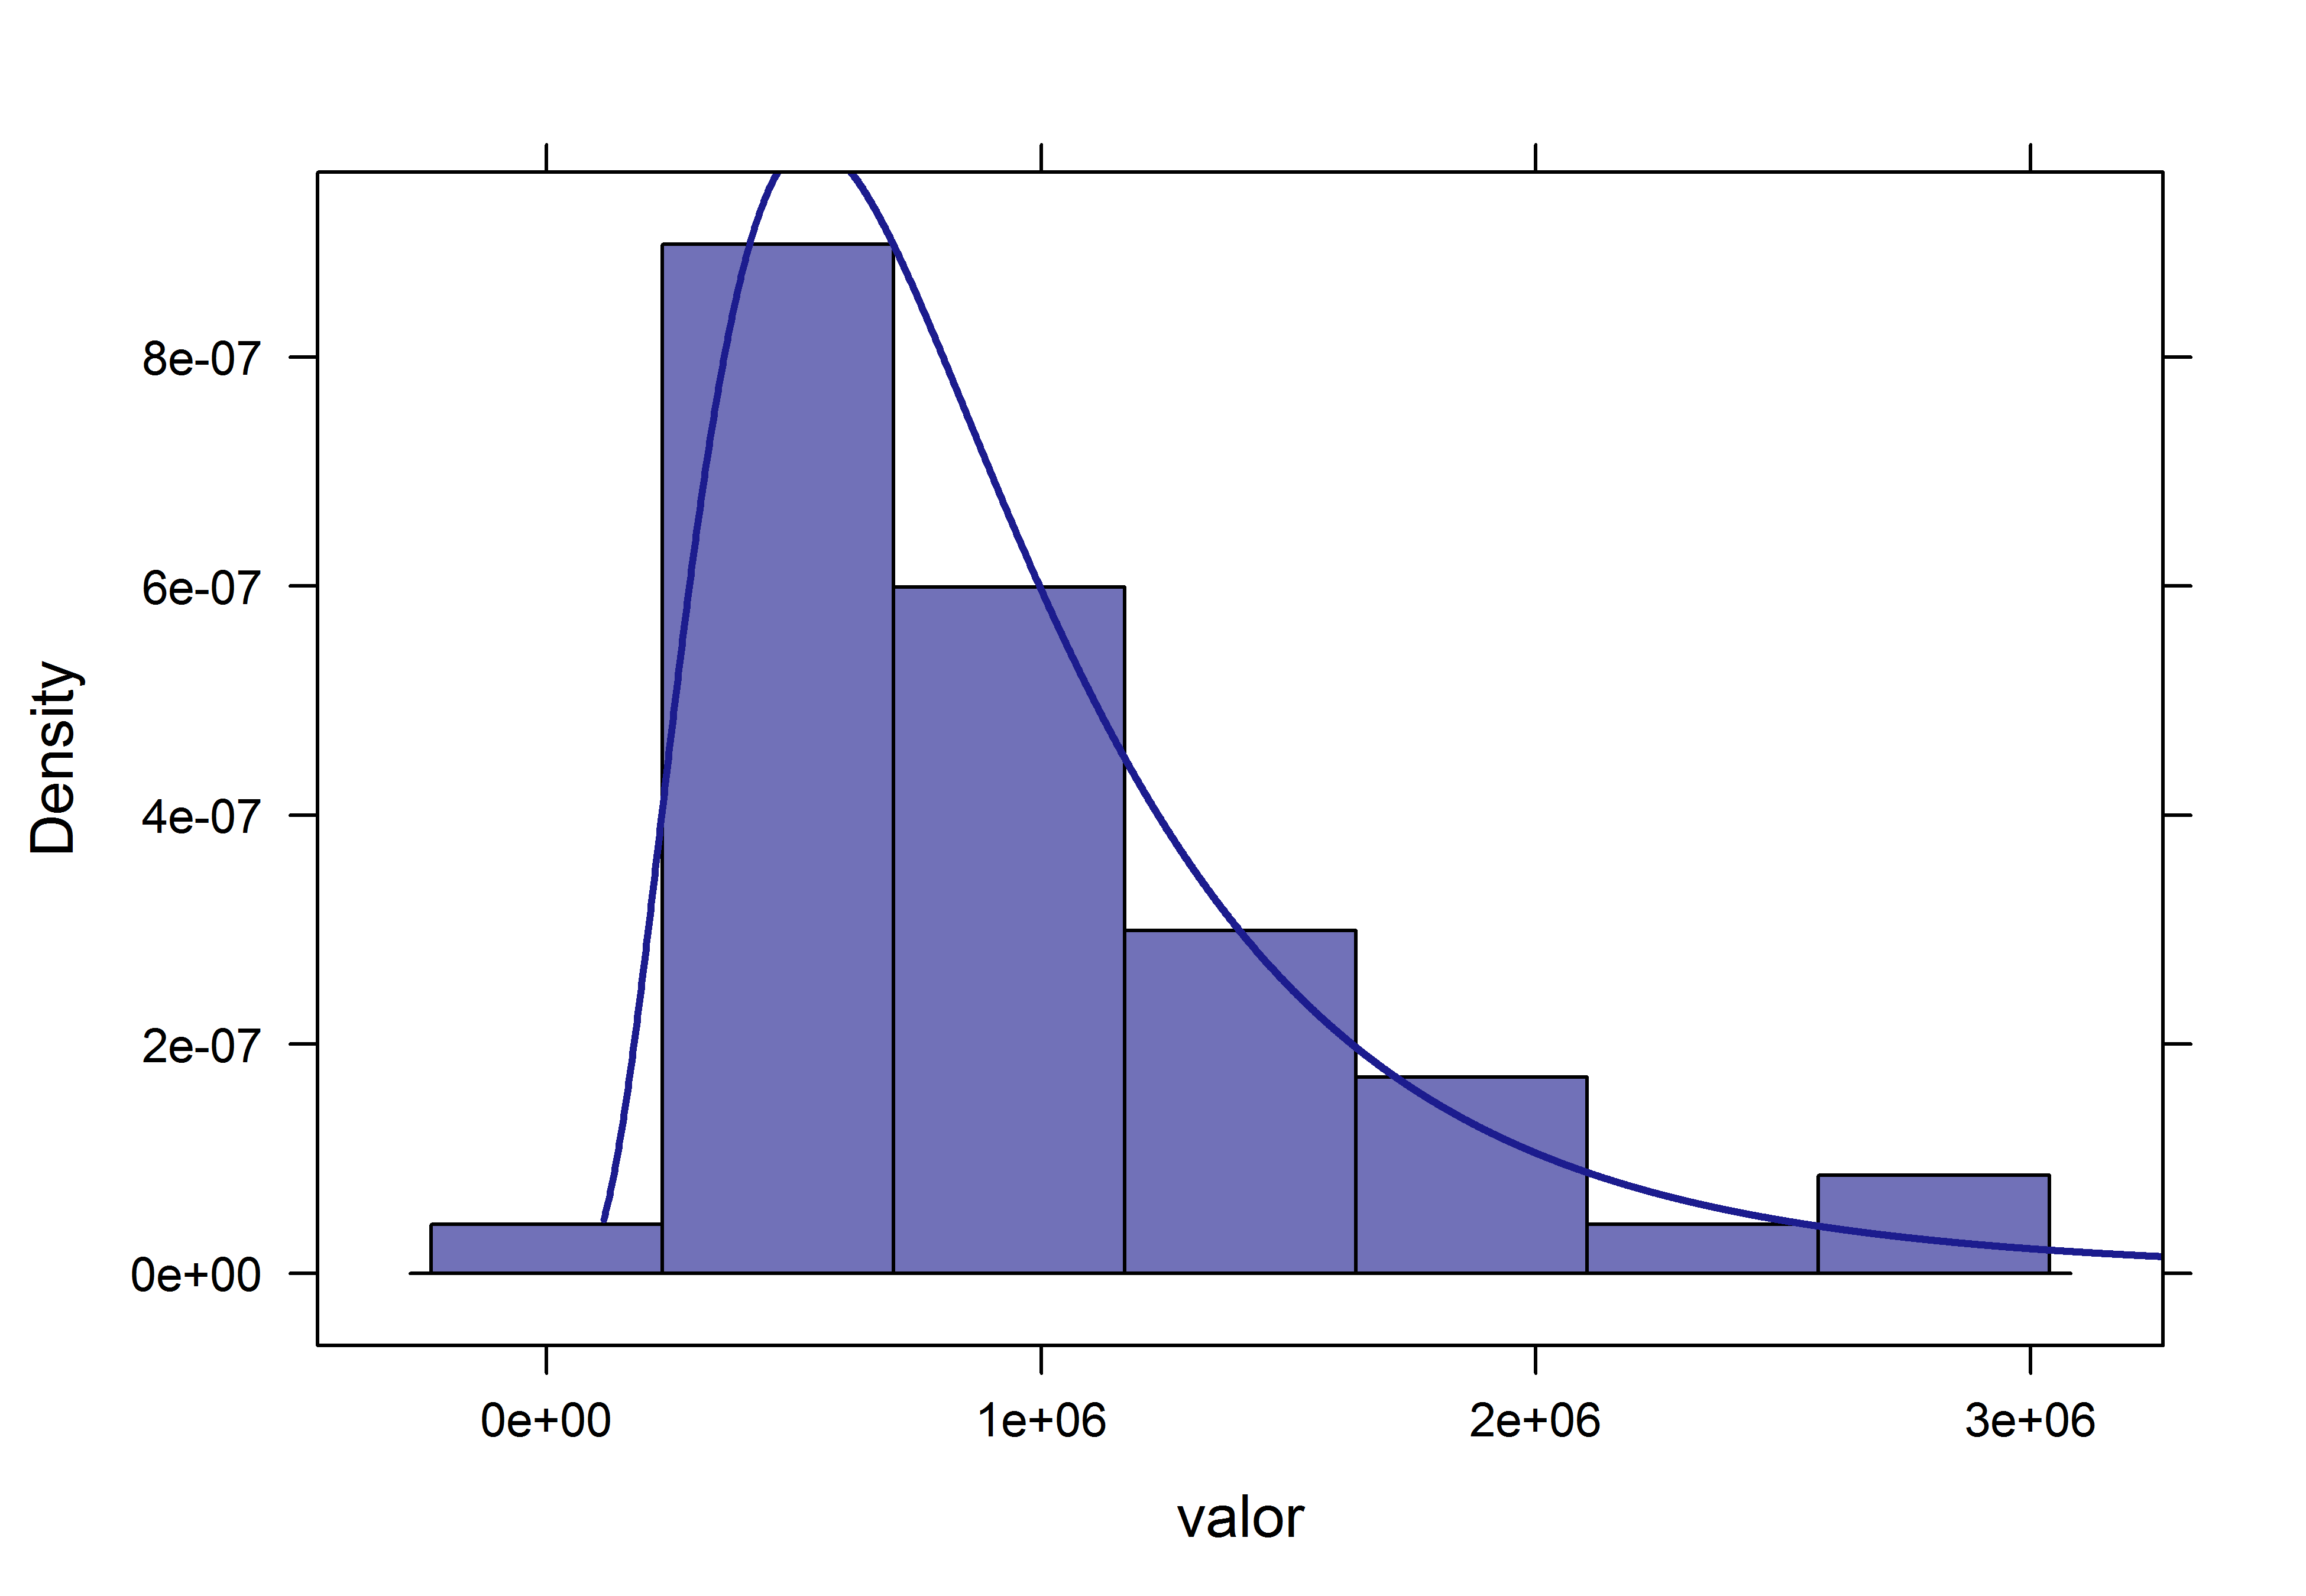
\includegraphics[width=0.5\linewidth]{images/hist_densidade-1} 

}

\caption{Histograma das variável \code{valor} com função densidade de probabilidade superposta.}\label{fig:hist_densidade}
\end{figure}

\begin{enumerate}
\def\labelenumi{\alph{enumi}.}
\setcounter{enumi}{2}
\tightlist
\item
  Cumulativa
\end{enumerate}

A figura \ref{fig:cdf} ilustra o gráfico da função cumulativa de
probabilidade (FCP) para a variável \texttt{valor}.

\begin{figure}[H]

{\centering 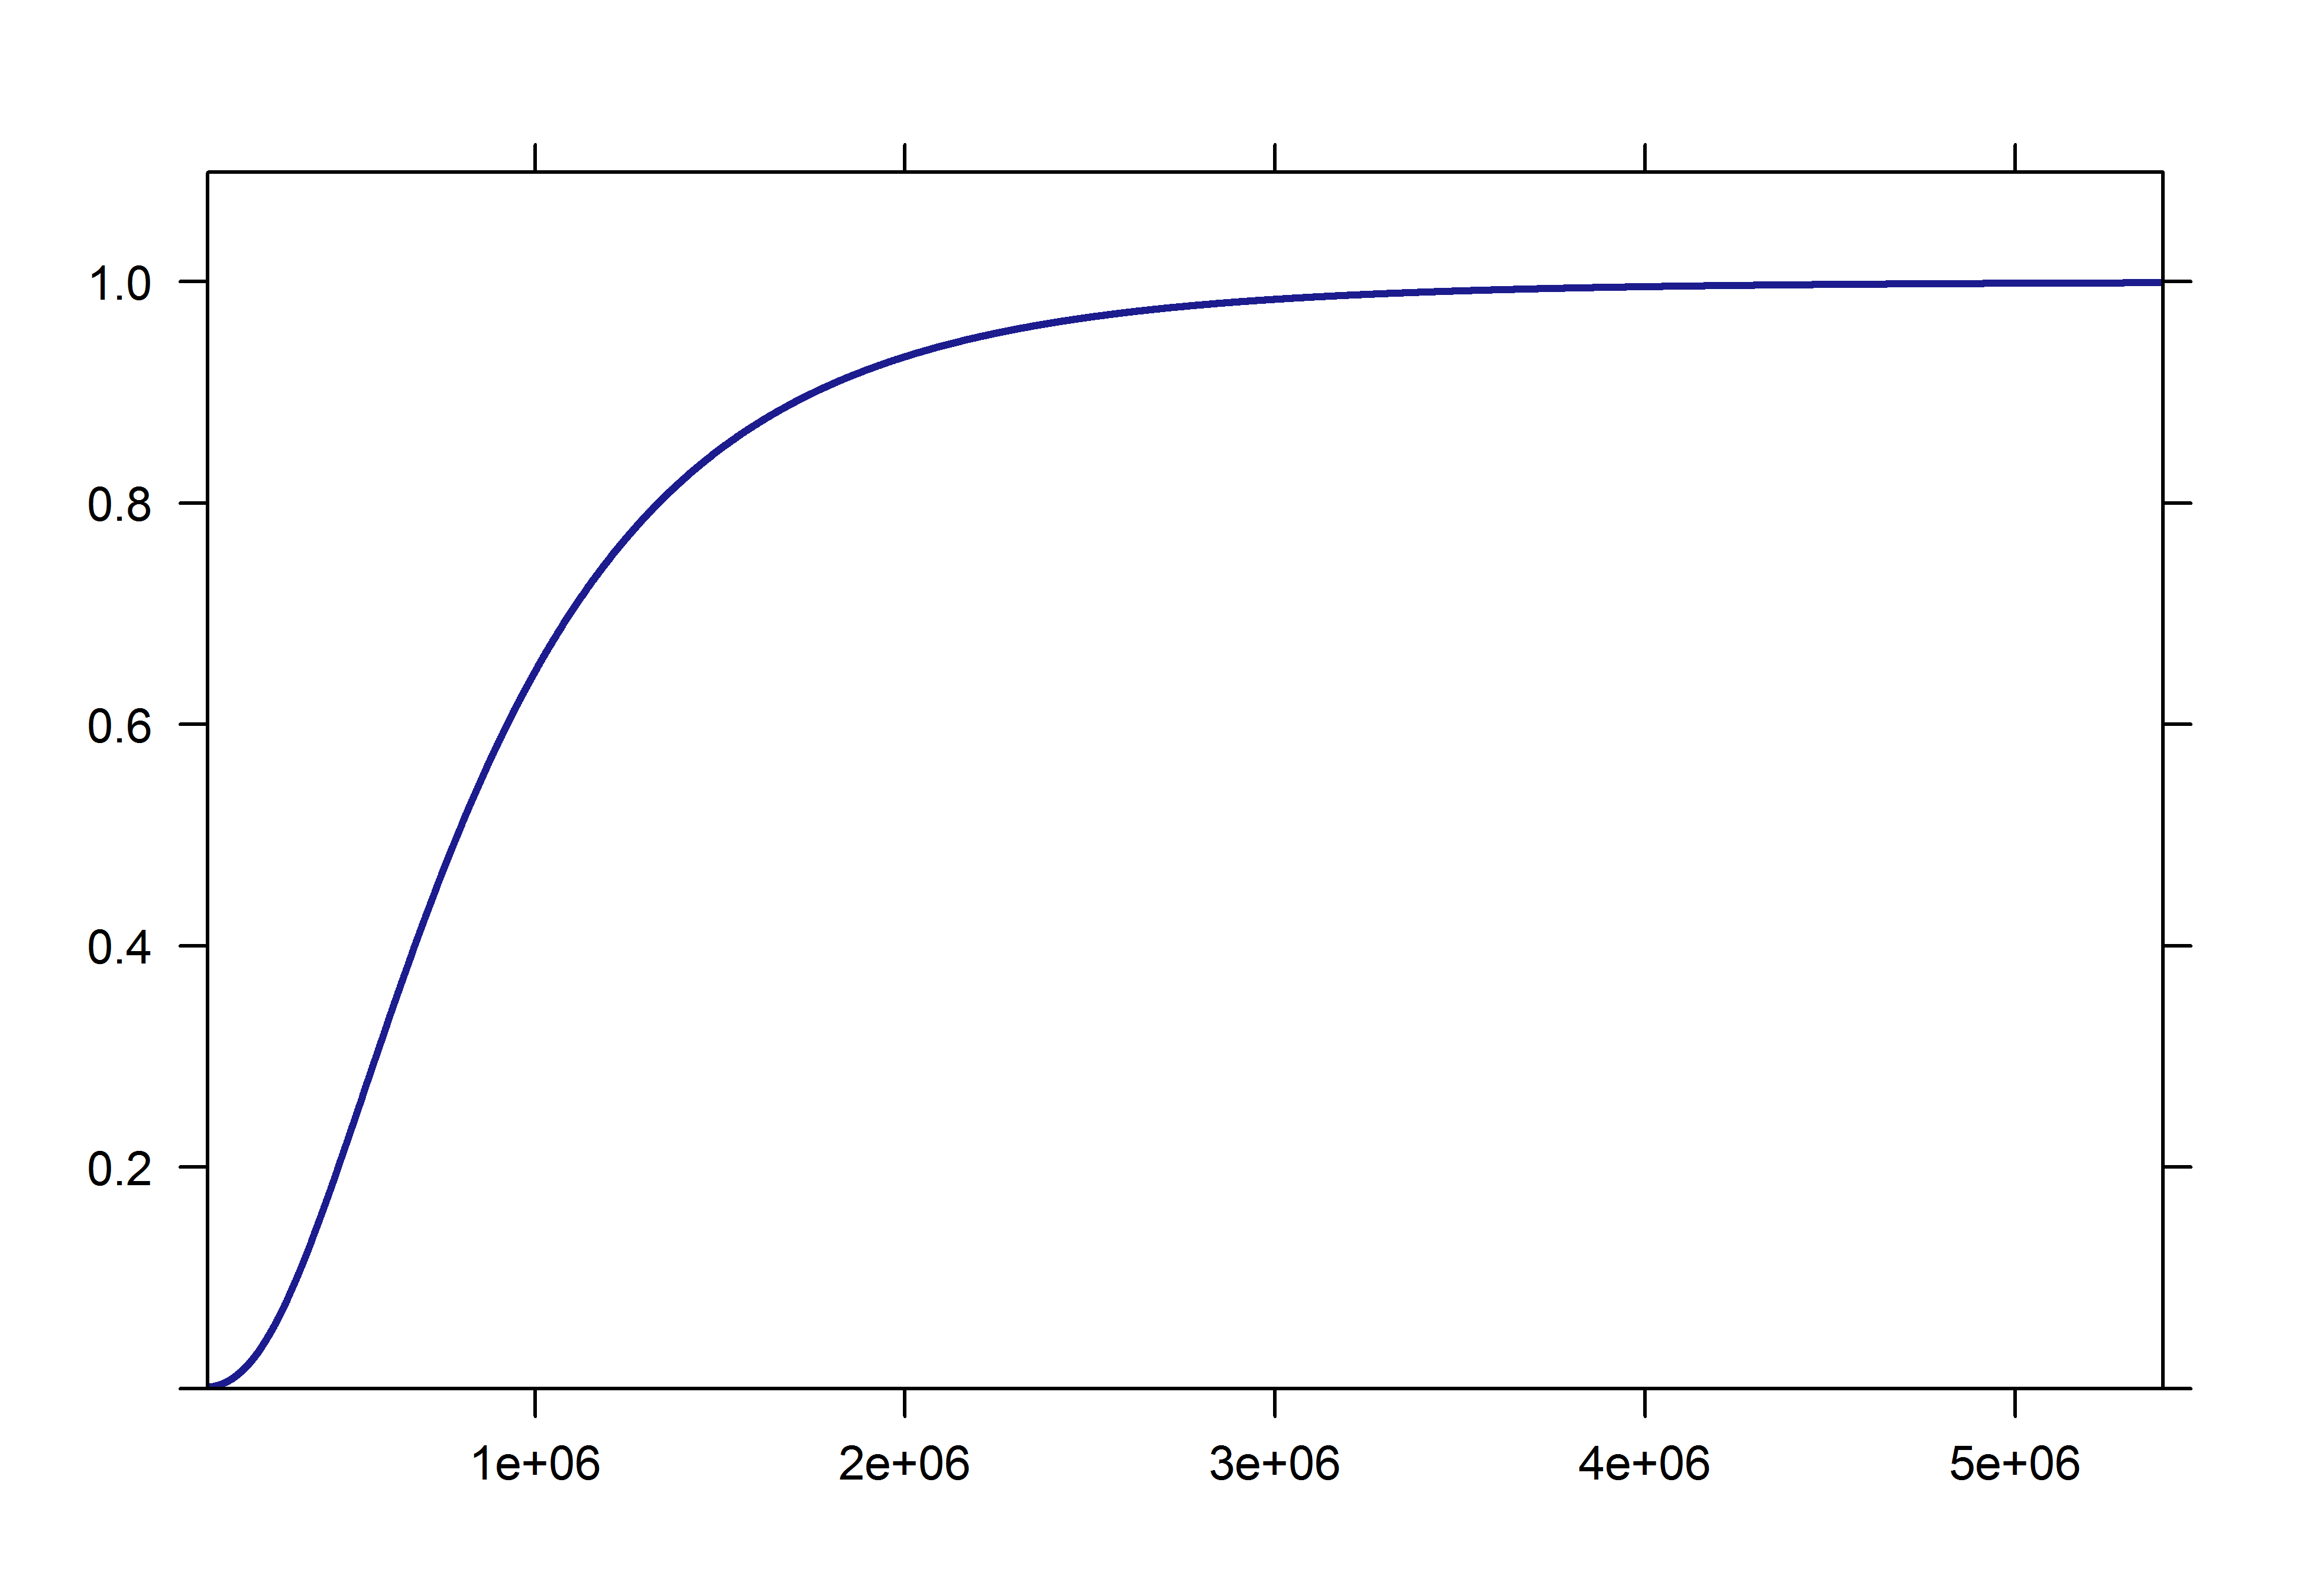
\includegraphics[width=0.5\linewidth]{images/cdf-1} 

}

\caption{Função cumulativa de densidade de probabilidade com parâmetros obtidos dos dados da variável \code{valor}}\label{fig:cdf}
\end{figure}

\begin{enumerate}
\def\labelenumi{\alph{enumi}.}
\setcounter{enumi}{3}
\tightlist
\item
  Distribuição da variável \(ln(valor)\)
\end{enumerate}

A figura \ref{fig:hist_densidade2} mostra a distribuição da variável
\(\ln(valor)\). Pode-se notar que, conforme esperado, já que a
distribuição da variável \texttt{valor} é aproximadamente lognormal, seu
logaritmo tem distribuição aproximadamente normal.

\begin{figure}[H]

{\centering 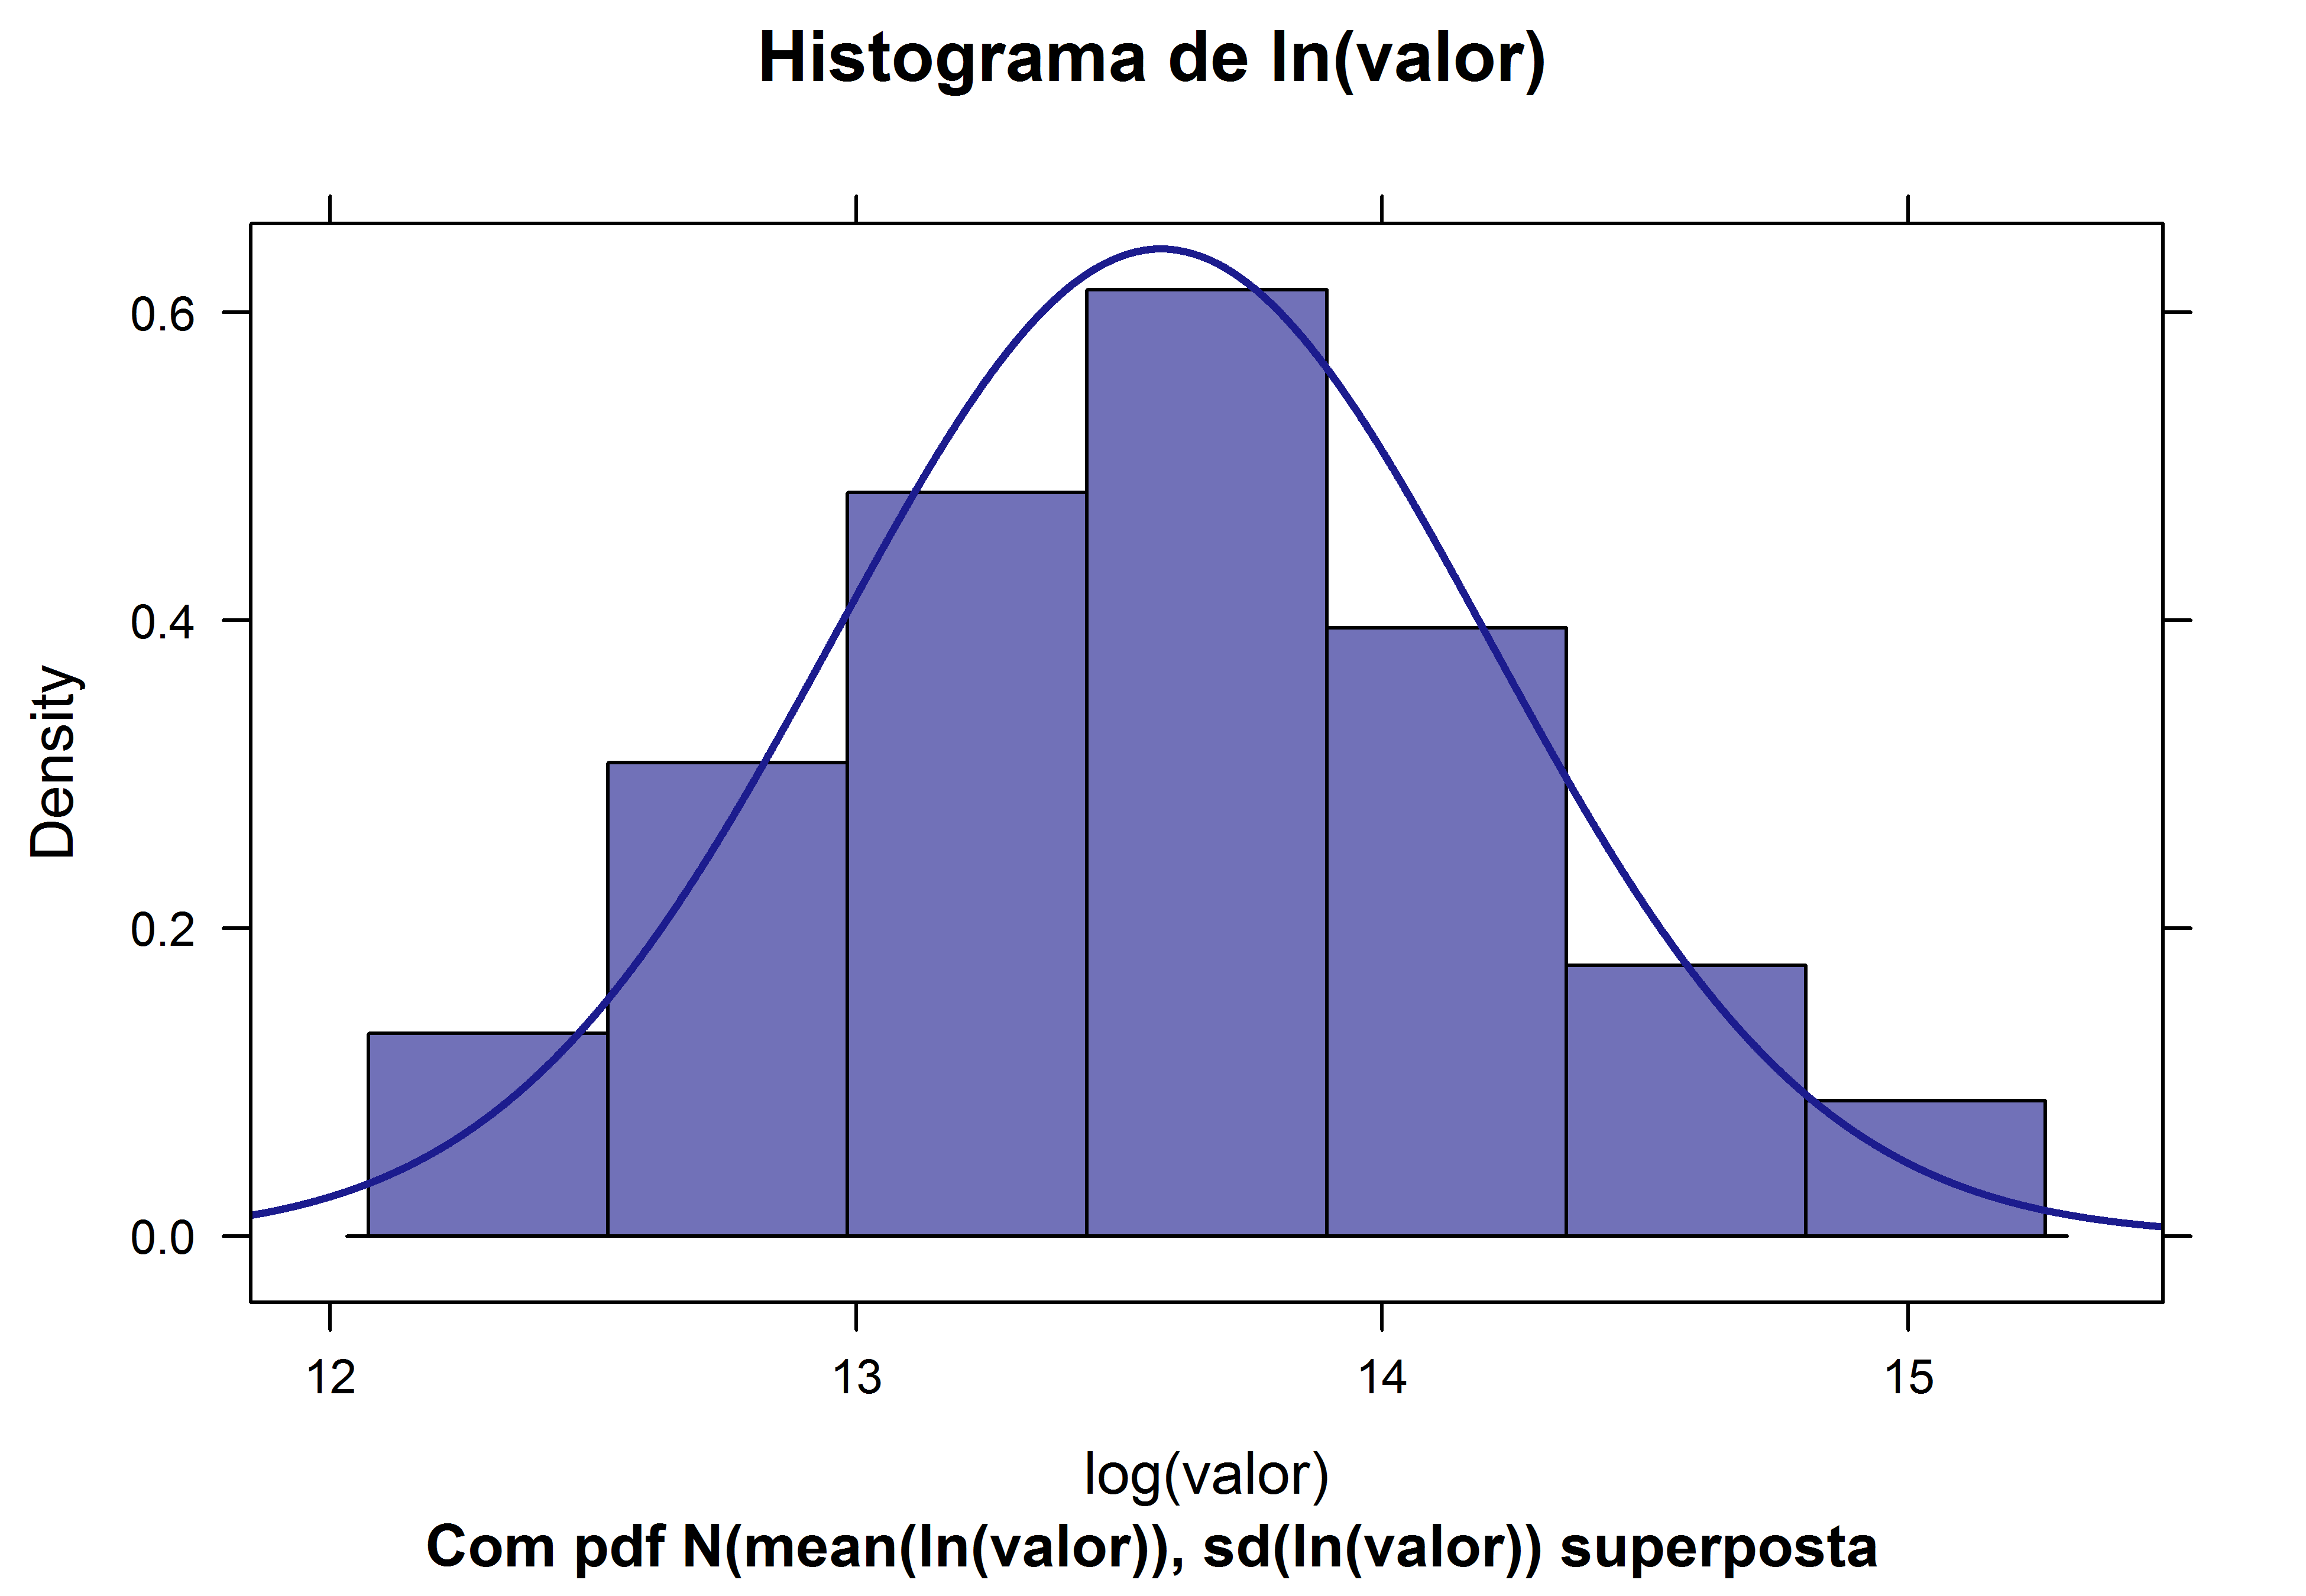
\includegraphics[width=0.5\linewidth]{images/hist_densidade2-1} 

}

\caption{Histograma com função densidade de probabilidade normal superposta}\label{fig:hist_densidade2}
\end{figure}

\subsection{Modelos}\label{modelos}

Detectando-se a presença de variável resposta com distribuição
lognormal, pode-se proceder da seguinte maneira:

\begin{itemize}
\tightlist
\item
  Proceder com a transformação da variável resposta pela função
  logarítmica;
\item
  Proceder com a variável na escala original, corrigindo posteriormente
  a heteroscedasticidade com o método de Eickert-White;
\item
  Proceder com o Método dos Mínimos Quadrados Ponderados.
\end{itemize}

\subsubsection{Modelo linear com a variável resposta
transformada}\label{modelo-linear-com-a-variavel-resposta-transformada}

É fácil mostrar que o modelo linear com a variável resposta
logaritmizada, ou seja, com distribuição normal, é melhor ajustado que o
modelo linear de uma variável resposta lognormal. Na tabela
\ref{tab:tabela}, no entanto, mostra-se que, para o presente caso, esta
melhora de ajuste é modesta, próxima a 4,5\%. Além disso, o modelo
linear, sem transformação, é heteroscedástico.

\begin{verbatim}
## 
##  studentized Breusch-Pagan test
## 
## data:  fit
## BP = 17.882753, df = 7, p-value = 0.01251035
\end{verbatim}

A função máxima verossimilhança de Box-Cox também vai apresentar como
transformação ótima a transformação logarítimica, como demonstra a
figura \ref{fig:boxcox}

\begin{figure}[H]

{\centering 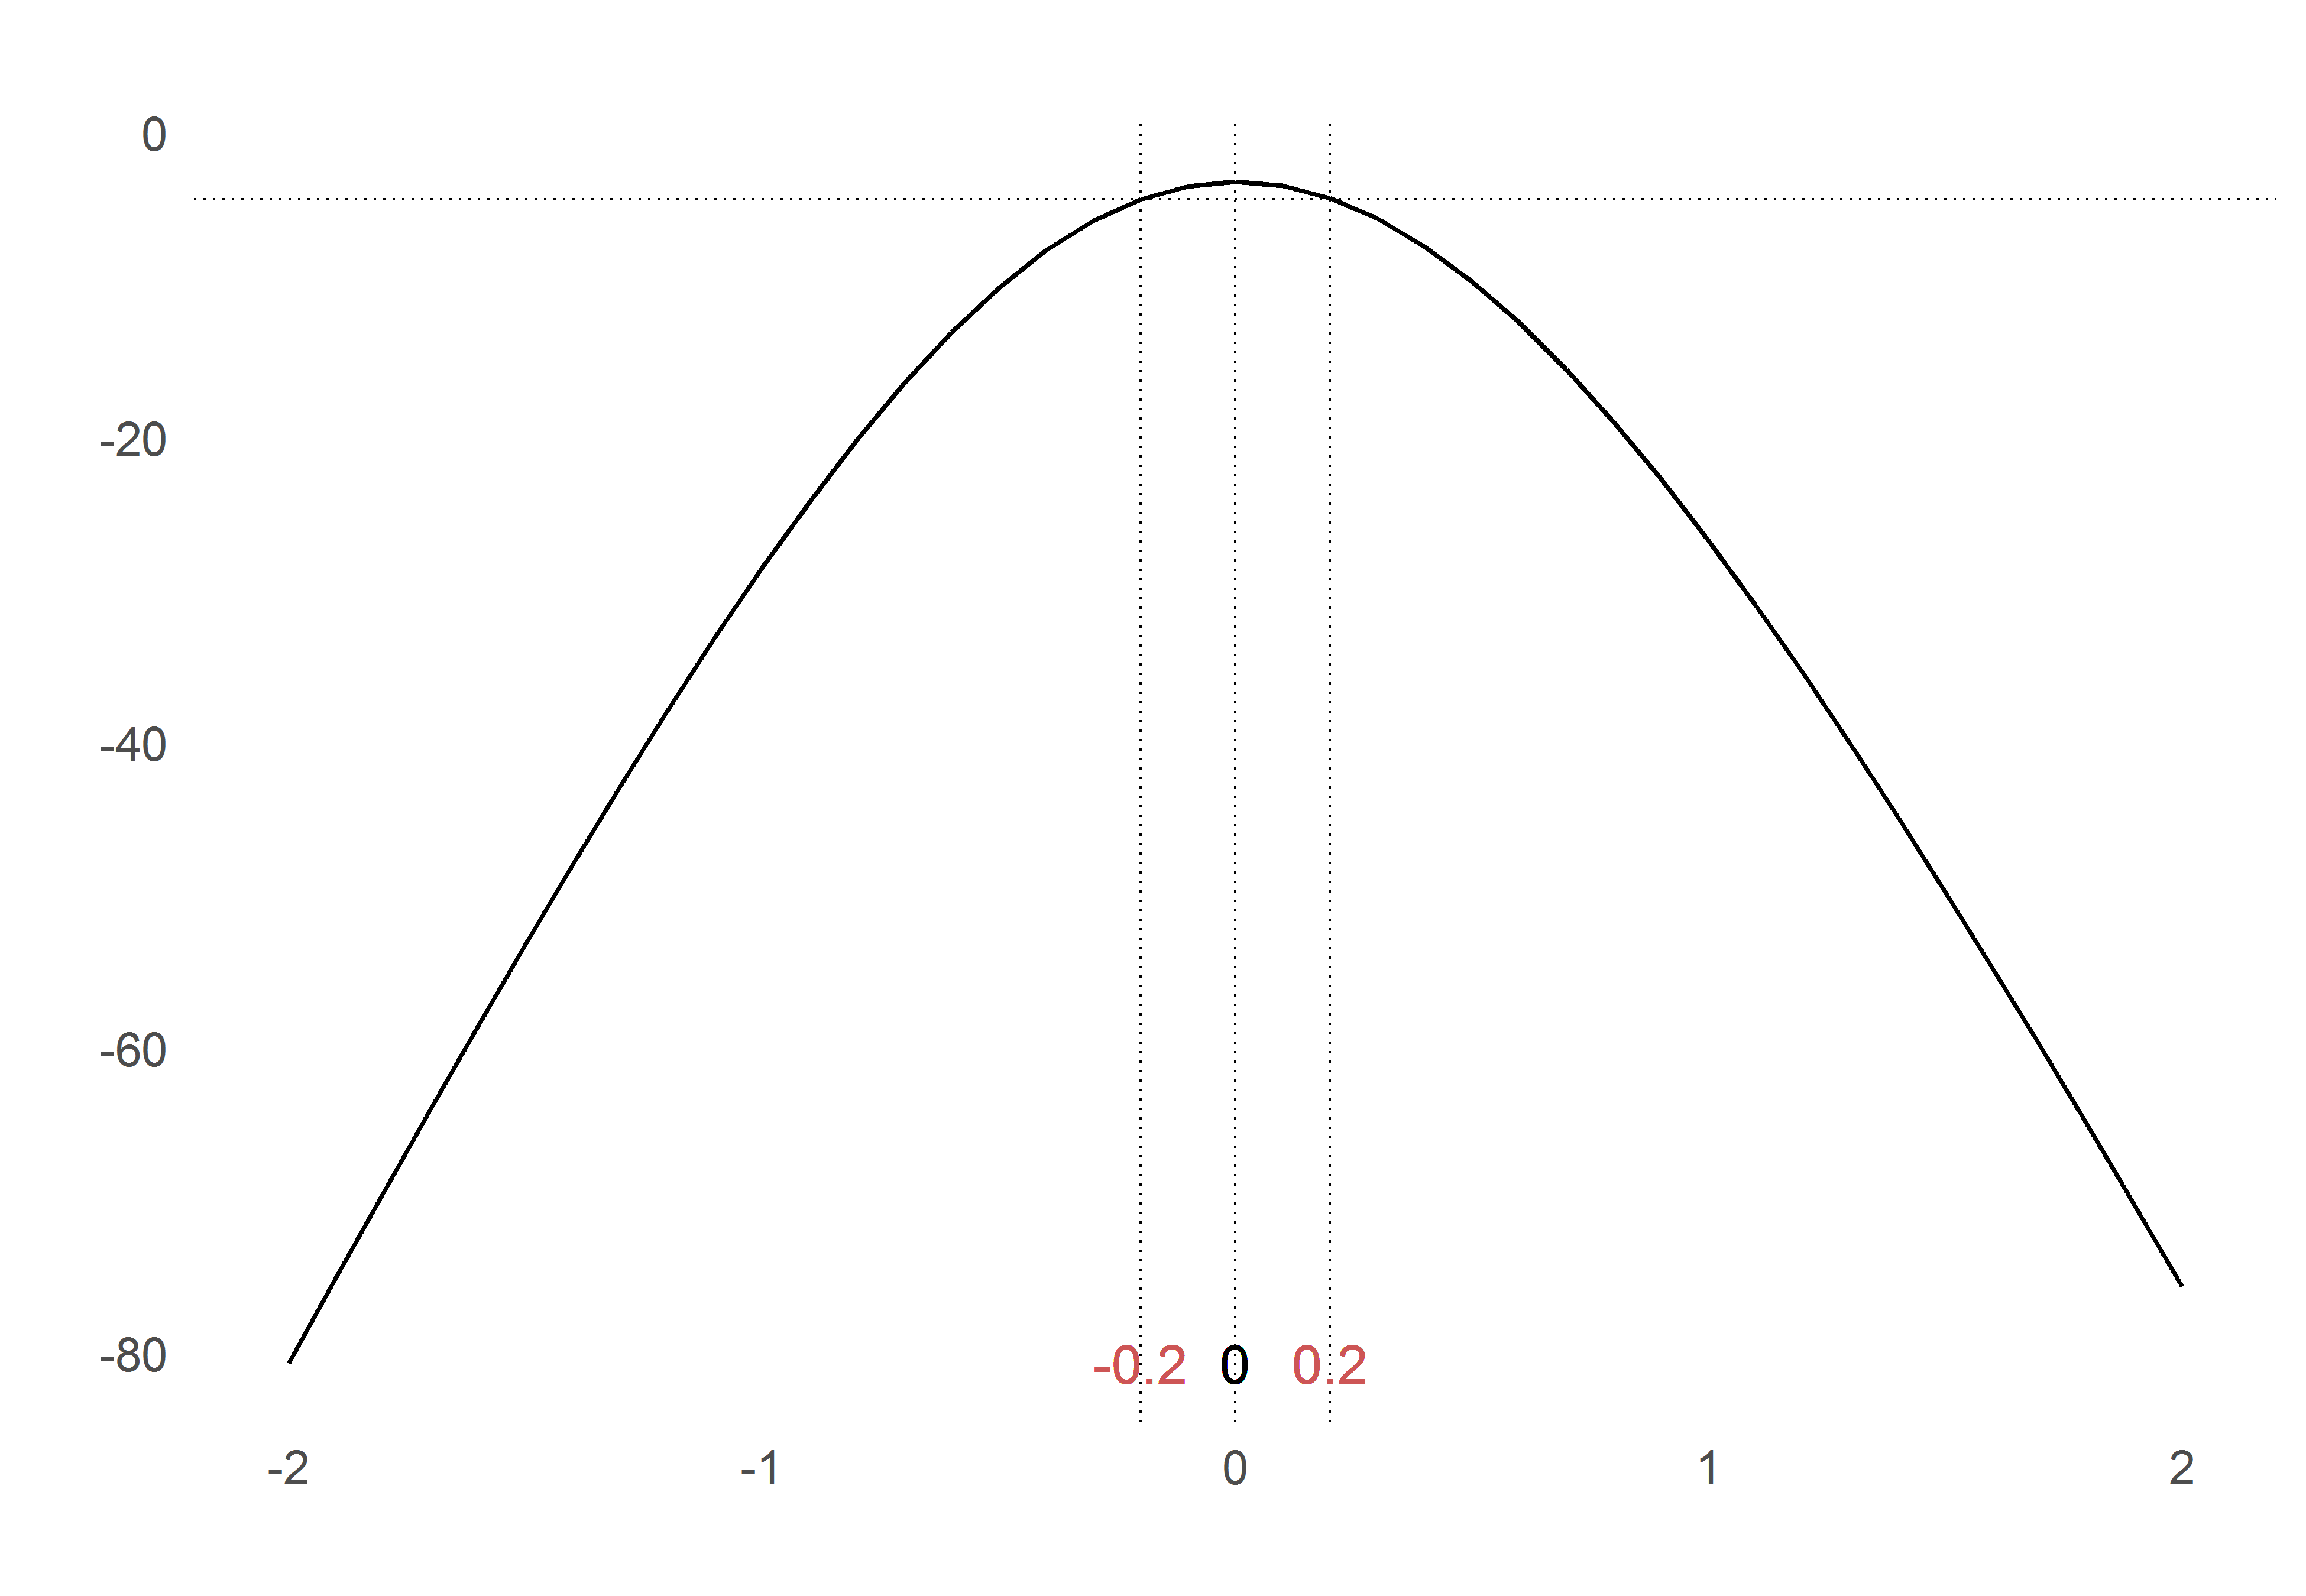
\includegraphics[width=0.5\linewidth]{images/boxcox-1} 

}

\caption{Gráfico da função verossimilhança de Box-Cox}\label{fig:boxcox}
\end{figure}

Na tabela \ref{tab:tabela} é possível comparar os modelos com e sem a
transformação da variável resposta. Porém, como o modelo sem
transformação é heteroscedástico, os intervalos de confiança dos
regressores e os p-valores mostrados na tabela são inválidos, pois
deve-se calcular os erros robustos antes de computá-los, o que será
visto na próxima seção.

\begin{table}[!htbp] \centering 
  \caption{Comparação entre modelos com e sem transformação da variável resposta} 
  \label{tab:tabela} 
\begin{tabular}{@{\extracolsep{5pt}}lcc} 
\\[-1.8ex]\hline 
\hline \\[-1.8ex] 
 & \multicolumn{2}{c}{\textit{Dependent variable:}} \\ 
\cline{2-3} 
\\[-1.8ex] & valor & log(valor) \\ 
\\[-1.8ex] & (1) & (2)\\ 
\hline \\[-1.8ex] 
 area\_total & 2,893.178 & 0.002 \\ 
  & (2,065.405, 3,720.951) & (0.001, 0.002) \\ 
  & t = 6.850 & t = 4.886 \\ 
  & p = 0.00000$^{***}$ & p = 0.00002$^{***}$ \\ 
  & & \\ 
 quartos & 73,524.375 & 0.169 \\ 
  & ($-$34,814.143, 181,862.894) & (0.084, 0.255) \\ 
  & t = 1.330 & t = 3.870 \\ 
  & p = 0.191 & p = 0.0004$^{***}$ \\ 
  & & \\ 
 suites & 111,000.591 & 0.088 \\ 
  & (8,045.131, 213,956.052) & (0.007, 0.170) \\ 
  & t = 2.113 & t = 2.121 \\ 
  & p = 0.041$^{**}$ & p = 0.040$^{**}$ \\ 
  & & \\ 
 garagens & 148,427.448 & 0.175 \\ 
  & (49,657.102, 247,197.795) & (0.097, 0.253) \\ 
  & t = 2.945 & t = 4.394 \\ 
  & p = 0.006$^{***}$ & p = 0.0001$^{***}$ \\ 
  & & \\ 
 dist\_b\_mar & $-$223.217 & $-$0.0003 \\ 
  & ($-$434.862, $-$11.571) & ($-$0.0004, $-$0.0001) \\ 
  & t = $-$2.067 & t = $-$3.215 \\ 
  & p = 0.045$^{**}$ & p = 0.003$^{***}$ \\ 
  & & \\ 
 padraomedio & $-$146,549.393 & 0.268 \\ 
  & ($-$354,850.457, 61,751.672) & (0.103, 0.433) \\ 
  & t = $-$1.379 & t = 3.190 \\ 
  & p = 0.176 & p = 0.003$^{***}$ \\ 
  & & \\ 
 padraoalto & $-$56,064.550 & 0.334 \\ 
  & ($-$264,003.525, 151,874.426) & (0.169, 0.498) \\ 
  & t = $-$0.528 & t = 3.975 \\ 
  & p = 0.600 & p = 0.0003$^{***}$ \\ 
  & & \\ 
 Constant & 33,953.788 & 12.315 \\ 
  & ($-$267,469.800, 335,377.375) & (12.076, 12.553) \\ 
  & t = 0.221 & t = 101.170 \\ 
  & p = 0.827 & p = 0.000$^{***}$ \\ 
  & & \\ 
\hline \\[-1.8ex] 
Observations & 50 & 50 \\ 
R$^{2}$ & 0.906 & 0.940 \\ 
Adjusted R$^{2}$ & 0.890 & 0.930 \\ 
Akaike Inf. Crit. & 1,375.659 & $-$29.275 \\ 
Residual Std. Error (df = 42) & 207,903.003 & 0.165 \\ 
F Statistic (df = 7; 42) & 57.731$^{***}$ & 94.063$^{***}$ \\ 
\hline 
\hline \\[-1.8ex] 
\textit{Note:}  & \multicolumn{2}{r}{$^{*}$p$<$0.1; $^{**}$p$<$0.05; $^{***}$p$<$0.01} \\ 
\end{tabular} 
\end{table}

\subsection{Retransformação de
variáveis}\label{retransformacao-de-variaveis}

O problema da transformação da variável resposta no logarítmo da
variável resposta original, é que devemos estudar como proceder na
retranformação da variável, para efetuar a avaliação do imóvel.

\subsubsection{A desigualdade de Jensen}\label{a-desigualdade-de-jensen}

Segundo Matloff (\protect\hyperlink{ref-matloff2017}{2017}, p. 142), a
desigualdade de Jensen (aplicada à estatística) se traduz na seguinte
expressão, válida para funções convexas:

\[\mathbb{E}[h(V)] \geq h(\mathbb{E}[V])\]

Isto aplicado no caso da transformação logarítimica, que é uma função
côncava, se reduz à expressão abaixo (MATLOFF,
\protect\hyperlink{ref-matloff2017}{2017}, p. 142):

\[\mathbb{E}[\ln Y|X = t] \leq \ln(E[Y|X = t])\]

Para Matloff, então, como a igualdade só irá acontecer em poucos casos
especiais, a função de regressão de \(\ln(Y)\) será quase sempre menor
do que o logaritmo natural da função de regressão de \(Y\), de tal forma
que a suposição que dado uma variável aleatória \(Y\) tal que assumimos
que \(E(Y|X = t) = e^{\beta_0 + \beta_1t}\), não podemos concluir de
imediato que um modelo linear razoável seria da forma
\(E(\ln Y|X = t) = \beta_0 + \beta_1t\), pois, pela desigualdade de
Jensen, se temos dados significantemente heteroscedásticos da variável
original (\(Y\)), a discrepância entre os dois lados da desigualdade
acima poderia variar bastante com \(t\), potencialmente produzindo uma
grande distorção à forma da curva de regressão (MATLOFF,
\protect\hyperlink{ref-matloff2017}{2017}, p. 143). Segundo Becker
(\protect\hyperlink{ref-becker}{2012}, p. 4), a desigualdade de Jensen
pode ser transformada numa igualdade do tipo:

\[\mathbb{E}[f(X)] = f(\mathbb{E}[X]) + \Delta\] E, de acordo com o
mesmo (\protect\hyperlink{ref-becker}{2012}, p. 5), o valor de
\(\Delta\), chamado de Defeito de Holder, é proporcional à variância da
variável aleatória \(X\), tal que se
\(f: [a, b] \rightarrow \mathbb{R}\) é duas vezes continuamente
diferenciável e existem limites finitos \(m\) e \(M\) tais que
\(0 \leq m \leq f''(x) \leq M\) para todo \(x \in [a,b]\), então existe
um valor \(\mu \in [m, M]\) para o qual a fórmula abaixo é válida:

\[\mathbb{E}[f(X)] - f(\mathbb{E}[X]) = \frac{1}{2}\mu \mathrm{Var} (X)\]
Em suma, o valor de \(\Delta\) é proporcional à variância de \(X\)
(\(\Delta \propto \sigma^2(X)\)).

Deste modo, existem na literatura diversos estudos sobre qual seria o
``melhor'' estimador -- paramétrico ou não-paramétrico -- para a
variável resposta original, quando da ocorrência da transformação da
variável pela função logaritmo natural, como pode ser visto em DUAN
(\protect\hyperlink{ref-Duan}{1983}), MEULENBERG
(\protect\hyperlink{ref-meulenberg1965}{1965}) e SHEN; ZHU
(\protect\hyperlink{ref-shen}{2008}).

De acordo com Shen e Zhu (\protect\hyperlink{ref-shen}{2008}), com a
simples aplicação da transformação inversa (exponencial) à aplicada na
variável dependente (logarítimica), chegamos ao \emph{Back-Transform}
(BT) \emph{Estimator}, que tem performance ``muito pior do que os outros
estimadores'' (\protect\hyperlink{ref-shen}{2008}, p. 554). De fato, o
estimador BT seria mais apropriado para estimar a mediana (SHEN; ZHU,
\protect\hyperlink{ref-shen}{2008}, p. 554), no entanto a equação de
regressão linear é uma equação para a média da variável dependente.
Métodos de regressão à mediana (KOENKER; HALLOCK,
\protect\hyperlink{ref-koenker}{2001}), então, seriam mais apropriados
para este fim.

Entendemos que, na precisão necessária para a área de avaliação de
imóveis, é suficiente a adoção do estimador teórico, apesar do
funcionamento dos estimadores não-paramétricos ter sido demonstrado mais
eficiente do que ele.

\[\mathbb{E}(Y|X) = \exp(\beta_0 + \beta_1X + 0.5\sigma^2)\]

\subsubsection{Modelo linear com posterior correção da
heteroscedasticidade}\label{modelo-linear-com-posterior-correcao-da-heteroscedasticidade}

\paragraph{Erros-padrão robustos}\label{erros-padrao-robustos}

\begin{enumerate}
\def\labelenumi{\alph{enumi}.}
\tightlist
\item
  Coeficientes
\end{enumerate}

\begin{table}[!htbp] \centering 
  \caption{Comparação entre modelos com e sem erros robustos} 
  \label{tab:tabela2} 
\begin{tabular}{@{\extracolsep{5pt}}lcc} 
\\[-1.8ex]\hline 
\hline \\[-1.8ex] 
 & \multicolumn{2}{c}{\textit{Dependent variable:}} \\ 
\cline{2-3} 
\\[-1.8ex] & \multicolumn{2}{c}{valor} \\ 
 & default & robust \\ 
\\[-1.8ex] & (1) & (2)\\ 
\hline \\[-1.8ex] 
 area\_total & 2.893,178 & 2.893,178 \\ 
  & (2.065,405, 3.720,951) & (1.712,055, 4.074,302) \\ 
  & t = 6,850 & t = 4,801 \\ 
  & p = 0,00000$^{***}$ & p = 0,00001$^{***}$ \\ 
  & & \\ 
 quartos & 73.524,375 & 73.524,375 \\ 
  & ($-$34.814,143, 181.862,894) & ($-$31.897,755, 178.946,506) \\ 
  & t = 1,330 & t = 1,367 \\ 
  & p = 0,191 & p = 0,172 \\ 
  & & \\ 
 suites & 111.000,591 & 111.000,591 \\ 
  & (8.045,131, 213.956,052) & (18.671,249, 203.329,934) \\ 
  & t = 2,113 & t = 2,356 \\ 
  & p = 0,041$^{**}$ & p = 0,019$^{**}$ \\ 
  & & \\ 
 garagens & 148.427,448 & 148.427,448 \\ 
  & (49.657,102, 247.197,795) & (73.906,905, 222.947,992) \\ 
  & t = 2,945 & t = 3,904 \\ 
  & p = 0,006$^{***}$ & p = 0,0001$^{***}$ \\ 
  & & \\ 
 dist\_b\_mar & $-$223,217 & $-$223,217 \\ 
  & ($-$434,862, $-$11,571) & ($-$406,588, $-$39,845) \\ 
  & t = $-$2,067 & t = $-$2,386 \\ 
  & p = 0,045$^{**}$ & p = 0,018$^{**}$ \\ 
  & & \\ 
 padraomedio & $-$146.549,393 & $-$146.549,393 \\ 
  & ($-$354.850,457, 61.751,672) & ($-$322.293,226, 29.194,441) \\ 
  & t = $-$1,379 & t = $-$1,634 \\ 
  & p = 0,176 & p = 0,103 \\ 
  & & \\ 
 padraoalto & $-$56.064,550 & $-$56.064,550 \\ 
  & ($-$264.003,525, 151.874,426) & ($-$197.646,893, 85.517,794) \\ 
  & t = $-$0,528 & t = $-$0,776 \\ 
  & p = 0,600 & p = 0,438 \\ 
  & & \\ 
 Constant & 33.953,788 & 33.953,788 \\ 
  & ($-$267.469,800, 335.377,375) & ($-$191.823,586, 259.731,161) \\ 
  & t = 0,221 & t = 0,295 \\ 
  & p = 0,827 & p = 0,769 \\ 
  & & \\ 
\hline \\[-1.8ex] 
Observations & 50 & 50 \\ 
R$^{2}$ & 0,906 & 0,906 \\ 
Adjusted R$^{2}$ & 0,890 & 0,890 \\ 
Akaike Inf. Crit. & 1.375,659 & 1.375,659 \\ 
Residual Std. Error (df = 42) & 207.903,003 & 207.903,003 \\ 
F Statistic (df = 7; 42) & 57,731$^{***}$ & 57,731$^{***}$ \\ 
\hline 
\hline \\[-1.8ex] 
\textit{Note:}  & \multicolumn{2}{r}{$^{*}$p$<$0,1; $^{**}$p$<$0,05; $^{***}$p$<$0,01} \\ 
\end{tabular} 
\end{table}

\begin{enumerate}
\def\labelenumi{\alph{enumi}.}
\setcounter{enumi}{1}
\tightlist
\item
  Teste F
\end{enumerate}

Na tabela \ref{tab:tabela2}, o resultado para o teste F para o modelo
robusto está errado. O teste deve ser refeito com a consideração dos
erros robustos:

\begin{verbatim}
## Wald test
## 
## Model 1: valor ~ area_total + quartos + suites + garagens + dist_b_mar + 
##     padrao
## Model 2: valor ~ 1
##   Res.Df Df        F     Pr(>F)    
## 1     42                           
## 2     49 -7 33.42548 3.3877e-15 ***
## ---
## Signif. codes:  0 '***' 0.001 '**' 0.01 '*' 0.05 '.' 0.1 ' ' 1
\end{verbatim}

\subsubsection{Mínimos quadrados
ponderados}\label{minimos-quadrados-ponderados}

De acordo com Matloff (\protect\hyperlink{ref-matloff2017}{2017}, p.
139), em princípio, o Método dos Mínimos Quadrados ponderados (MQP)
fornece melhores estimativas para os coeficientes e inferência
estatística correta mesmo na presença de heteroscedasticidade. Tal
método consiste, analogamente ao Método dos Mínimos Quadrados Ordinários
(MQO), em uma minimização. No caso dos MQO, minimiza-se a quantidade
abaixo (MATLOFF, \protect\hyperlink{ref-matloff2017}{2017}, p. 69):

\[\frac{1}{n} \sum_{i=1}^{n} (Y_i - \tilde{X}_i'b)^2\]

Enquanto o MQP minimiza (MATLOFF,
\protect\hyperlink{ref-matloff2017}{2017}, p. 133):

\[\frac{1}{n} \sum_{i=1}^{n} \frac{1}{w_i} (Y_i - \tilde{X}_i'b)^2\]

Onde \(w_i = \sigma^2(X_i)\).

\subsubsection{Comparação das previsões para os dois
modelos}\label{comparacao-das-previsoes-para-os-dois-modelos}

\begin{table}

\centering
\begin{tabular}[t]{rrrr}
\toprule
fit & lwr & upr & amplitude\\
\midrule
1.106.966,61 & 1.012.097,40 & 1.210.728,40 & 0,18\\
665.565,24 & 624.364,31 & 709.484,96 & 0,13\\
889.515,06 & 839.323,09 & 942.708,54 & 0,12\\
778.638,69 & 732.296,73 & 827.913,31 & 0,12\\
926.373,32 & 826.896,03 & 1.037.817,93 & 0,23\\
\addlinespace
366.492,31 & 337.377,96 & 398.119,10 & 0,17\\
720.258,16 & 676.775,68 & 766.534,37 & 0,12\\
679.913,27 & 635.304,18 & 727.654,68 & 0,14\\
677.695,98 & 633.095,02 & 725.439,04 & 0,14\\
703.407,28 & 661.531,44 & 747.933,93 & 0,12\\
\addlinespace
855.019,06 & 805.611,95 & 907.456,25 & 0,12\\
743.187,12 & 699.766,15 & 789.302,39 & 0,12\\
747.511,83 & 703.804,25 & 793.933,73 & 0,12\\
479.030,46 & 425.602,14 & 539.165,94 & 0,24\\
685.488,30 & 640.831,29 & 733.257,28 & 0,13\\
\addlinespace
1.339.514,49 & 1.217.160,39 & 1.474.168,13 & 0,19\\
1.116.148,08 & 1.040.974,23 & 1.196.750,59 & 0,14\\
663.458,78 & 618.767,51 & 711.377,93 & 0,14\\
712.383,70 & 668.349,56 & 759.319,03 & 0,13\\
431.580,00 & 389.600,88 & 478.082,34 & 0,21\\
\addlinespace
243.707,09 & 218.091,05 & 272.331,87 & 0,22\\
483.061,17 & 436.055,79 & 535.133,57 & 0,21\\
629.182,10 & 579.007,59 & 683.704,53 & 0,17\\
778.457,88 & 730.734,27 & 829.298,28 & 0,13\\
720.258,16 & 676.775,68 & 766.534,37 & 0,12\\
\addlinespace
385.471,14 & 354.491,70 & 419.157,91 & 0,17\\
236.922,70 & 216.532,40 & 259.233,11 & 0,18\\
289.533,09 & 265.323,28 & 315.951,95 & 0,17\\
233.663,54 & 209.605,75 & 260.482,61 & 0,22\\
398.390,85 & 358.851,53 & 442.286,72 & 0,21\\
\addlinespace
660.321,06 & 621.395,99 & 701.684,44 & 0,12\\
465.669,76 & 433.446,51 & 500.288,54 & 0,14\\
1.582.956,13 & 1.443.690,00 & 1.735.656,62 & 0,18\\
2.532.821,47 & 2.218.551,51 & 2.891.609,49 & 0,27\\
970.590,45 & 911.737,58 & 1.033.242,29 & 0,13\\
\addlinespace
1.219.926,54 & 1.095.450,47 & 1.358.546,82 & 0,22\\
1.022.195,60 & 909.895,02 & 1.148.356,49 & 0,23\\
1.129.958,73 & 1.033.156,70 & 1.235.830,67 & 0,18\\
2.093.864,11 & 1.905.595,34 & 2.300.733,44 & 0,19\\
1.938.988,72 & 1.716.090,88 & 2.190.838,08 & 0,24\\
\addlinespace
1.506.487,83 & 1.389.422,95 & 1.633.415,93 & 0,16\\
3.464.954,28 & 3.132.699,80 & 3.832.447,71 & 0,20\\
1.178.021,65 & 1.080.266,41 & 1.284.622,95 & 0,17\\
695.650,38 & 633.799,37 & 763.537,29 & 0,19\\
653.267,76 & 595.450,52 & 716.698,95 & 0,19\\
\addlinespace
2.284.770,17 & 2.093.977,72 & 2.492.946,64 & 0,17\\
1.639.750,58 & 1.523.582,17 & 1.764.776,47 & 0,15\\
813.100,32 & 762.277,24 & 867.311,91 & 0,13\\
1.587.840,38 & 1.464.634,52 & 1.721.410,37 & 0,16\\
802.909,81 & 750.036,73 & 859.510,12 & 0,14\\
\bottomrule
\end{tabular}
\centering
\begin{tabular}[t]{rrrrr}
\toprule
predicted.value & se & ci.lower & ci.upper & amplitude\\
\midrule
1.367.729,29 & 121.445,88 & 1.212.090,13 & 1.523.368,45 & 0,23\\
614.058,83 & 54.198,28 & 544.600,94 & 683.516,72 & 0,23\\
899.907,02 & 44.247,13 & 843.202,04 & 956.611,99 & 0,13\\
801.067,23 & 58.642,85 & 725.913,40 & 876.221,07 & 0,19\\
910.856,15 & 108.475,03 & 771.839,81 & 1.049.872,49 & 0,31\\
\addlinespace
445.349,38 & 61.718,67 & 366.253,72 & 524.445,03 & 0,36\\
844.240,07 & 47.795,77 & 782.987,32 & 905.492,82 & 0,15\\
647.454,84 & 49.257,70 & 584.328,56 & 710.581,11 & 0,19\\
641.668,48 & 49.966,95 & 577.633,26 & 705.703,70 & 0,20\\
615.796,95 & 61.632,22 & 536.812,09 & 694.781,81 & 0,26\\
\addlinespace
875.975,41 & 44.110,21 & 819.445,89 & 932.504,92 & 0,13\\
710.610,82 & 56.922,62 & 637.661,54 & 783.560,10 & 0,21\\
767.022,76 & 56.073,26 & 695.161,99 & 838.883,53 & 0,19\\
655.918,20 & 107.651,38 & 517.957,41 & 793.878,99 & 0,42\\
661.920,73 & 47.597,42 & 600.922,18 & 722.919,27 & 0,18\\
\addlinespace
1.242.341,34 & 108.121,24 & 1.103.778,40 & 1.380.904,29 & 0,22\\
1.223.757,21 & 61.228,63 & 1.145.289,57 & 1.302.224,86 & 0,13\\
604.057,16 & 55.122,03 & 533.415,44 & 674.698,89 & 0,23\\
835.311,40 & 49.911,85 & 771.346,79 & 899.276,00 & 0,15\\
307.366,82 & 79.165,78 & 205.911,79 & 408.821,85 & 0,66\\
\addlinespace
78.379,08 & 94.599,79 & -42.855,43 & 199.613,58 & 3,09\\
461.765,08 & 84.768,27 & 353.130,17 & 570.399,99 & 0,47\\
596.760,46 & 68.128,11 & 509.450,77 & 684.070,14 & 0,29\\
886.986,78 & 42.970,19 & 831.918,26 & 942.055,30 & 0,12\\
844.240,07 & 47.795,77 & 782.987,32 & 905.492,82 & 0,15\\
\addlinespace
504.060,39 & 66.837,58 & 418.404,59 & 589.716,20 & 0,34\\
83.402,49 & 71.838,72 & -8.662,54 & 175.467,52 & 2,21\\
280.558,89 & 59.715,18 & 204.030,81 & 357.086,97 & 0,55\\
81.364,57 & 94.434,20 & -39.657,73 & 202.386,87 & 2,97\\
467.967,00 & 86.507,23 & 357.103,53 & 578.830,48 & 0,47\\
\addlinespace
564.457,10 & 56.308,33 & 492.295,07 & 636.619,13 & 0,26\\
274.076,97 & 69.882,36 & 184.519,13 & 363.634,81 & 0,65\\
1.768.995,08 & 111.873,30 & 1.625.623,68 & 1.912.366,48 & 0,16\\
2.479.966,48 & 222.667,45 & 2.194.606,66 & 2.765.326,29 & 0,23\\
997.748,07 & 49.717,14 & 934.033,00 & 1.061.463,15 & 0,13\\
\addlinespace
1.276.034,44 & 100.520,14 & 1.147.212,69 & 1.404.856,18 & 0,20\\
1.042.565,59 & 87.168,88 & 930.854,17 & 1.154.277,01 & 0,21\\
1.259.219,73 & 93.817,14 & 1.138.988,22 & 1.379.451,24 & 0,19\\
2.184.590,06 & 173.904,42 & 1.961.722,59 & 2.407.457,54 & 0,20\\
1.793.276,36 & 85.876,83 & 1.683.220,78 & 1.903.331,95 & 0,12\\
\addlinespace
1.599.384,62 & 95.170,47 & 1.477.418,76 & 1.721.350,49 & 0,15\\
2.645.448,68 & 166.903,78 & 2.431.552,88 & 2.859.344,49 & 0,16\\
1.332.218,83 & 95.661,56 & 1.209.623,61 & 1.454.814,05 & 0,18\\
780.688,00 & 92.301,01 & 662.399,50 & 898.976,50 & 0,30\\
647.921,80 & 88.743,75 & 534.192,11 & 761.651,49 & 0,35\\
\addlinespace
2.103.307,21 & 101.647,13 & 1.973.041,18 & 2.233.573,25 & 0,12\\
1.754.167,54 & 103.229,33 & 1.621.873,83 & 1.886.461,25 & 0,15\\
805.379,85 & 50.113,27 & 741.157,10 & 869.602,60 & 0,16\\
1.619.940,75 & 84.278,29 & 1.511.933,78 & 1.727.947,73 & 0,13\\
802.717,96 & 65.833,83 & 718.348,51 & 887.087,41 & 0,21\\
\bottomrule
\end{tabular}
\end{table}

\section{CONCLUSÃO}\label{conclusao}

Foi possível demonstrar de maneira gráfica que os dados da variável
valor apresentados se ajustam bem a uma distribuição lognormal
equivalente. Por definição, então, o logaritmo da variável possui
distribuição normal.

Consideramos que o valor mais provável para a variável resposta é o seu
Valor Esperado. Logo, a retransformação da variável deve ser feita para
a média da variável log-normal.

Uma alternativa seria a aplicação da regressão linear ponderada (ou
mínimos quadrados ponderados). No entanto, o método de Eickert-White
parece ser adequado e sua aplicação menos complexa do que o método de
regressão ponderada. \newpage

\hypertarget{anexo-i}{\section*{ANEXO I}\label{anexo-i}}
\addcontentsline{toc}{section}{ANEXO I}

\begin{table}[H]
\centering\rowcolors{2}{gray!6}{white}

\begin{tabular}{rrrrrrl}
\hiderowcolors
\toprule
valor & area\_total & quartos & suites & garagens & dist\_b\_mar & padrao\\
\midrule
\showrowcolors
1060000 & 350.00 & 3 & 1 & 2 & 720 & medio\\
510000 & 136.56 & 3 & 1 & 1 & 665 & medio\\
780000 & 164.77 & 3 & 1 & 2 & 415 & medio\\
550000 & 174.58 & 3 & 1 & 1 & 320 & medio\\
850000 & 123.01 & 3 & 1 & 3 & 895 & alto\\
\addlinespace
300000 & 89.83 & 2 & 0 & 1 & 645 & baixo\\
750000 & 174.00 & 2 & 1 & 2 & 860 & alto\\
650000 & 123.00 & 3 & 1 & 1 & 745 & alto\\
620000 & 121.00 & 3 & 1 & 1 & 745 & alto\\
740000 & 109.00 & 3 & 1 & 1 & 300 & medio\\
\addlinespace
770000 & 170.00 & 3 & 1 & 2 & 590 & medio\\
680000 & 141.00 & 3 & 1 & 1 & 290 & medio\\
850000 & 174.00 & 3 & 1 & 1 & 465 & medio\\
420000 & 105.00 & 3 & 1 & 0 & 60 & baixo\\
547000 & 128.00 & 3 & 1 & 1 & 745 & alto\\
\addlinespace
1600000 & 163.00 & 4 & 2 & 2 & 90 & alto\\
1320000 & 230.00 & 3 & 1 & 2 & 215 & alto\\
615000 & 108.00 & 3 & 1 & 1 & 745 & alto\\
705000 & 174.00 & 2 & 1 & 2 & 900 & alto\\
418000 & 85.00 & 1 & 0 & 1 & 620 & alto\\
\addlinespace
270000 & 71.00 & 2 & 0 & 0 & 1380 & baixo\\
418000 & 100.00 & 1 & 1 & 1 & 620 & alto\\
650000 & 90.00 & 2 & 1 & 1 & 215 & alto\\
700000 & 161.00 & 2 & 1 & 2 & 500 & alto\\
680000 & 174.00 & 2 & 1 & 2 & 860 & alto\\
\addlinespace
420000 & 76.00 & 2 & 1 & 1 & 700 & baixo\\
195000 & 48.00 & 1 & 0 & 0 & 730 & baixo\\
290000 & 66.00 & 1 & 0 & 1 & 745 & baixo\\
272000 & 50.00 & 1 & 0 & 1 & 1430 & baixo\\
430000 & 61.00 & 2 & 0 & 1 & 170 & baixo\\
\addlinespace
895000 & 109.00 & 3 & 1 & 1 & 530 & medio\\
450000 & 89.00 & 2 & 0 & 1 & 745 & medio\\
1950000 & 393.00 & 3 & 1 & 3 & 550 & alto\\
2150000 & 578.00 & 3 & 2 & 3 & 260 & alto\\
940000 & 182.00 & 3 & 1 & 2 & 200 & medio\\
\addlinespace
1400000 & 262.00 & 4 & 1 & 1 & 60 & alto\\
1090000 & 205.00 & 3 & 0 & 3 & 465 & medio\\
1272000 & 196.00 & 3 & 3 & 2 & 610 & alto\\
2800000 & 463.00 & 3 & 3 & 3 & 590 & alto\\
1796000 & 273.00 & 3 & 3 & 4 & 140 & medio\\
\addlinespace
1400000 & 330.00 & 4 & 2 & 2 & 655 & alto\\
3000000 & 533.00 & 4 & 3 & 4 & 427 & alto\\
1200000 & 221.00 & 3 & 3 & 2 & 607 & alto\\
800000 & 220.00 & 3 & 1 & 1 & 1000 & medio\\
950000 & 127.00 & 2 & 1 & 1 & 60 & medio\\
\addlinespace
2061000 & 362.00 & 3 & 3 & 4 & 310 & alto\\
1326000 & 315.00 & 3 & 3 & 3 & 600 & alto\\
850000 & 151.00 & 3 & 1 & 2 & 660 & medio\\
1650000 & 246.00 & 3 & 3 & 3 & 307 & alto\\
650000 & 159.72 & 3 & 1 & 1 & 120 & medio\\
\bottomrule
\end{tabular}
\rowcolors{2}{white}{white}
\end{table}

\section*{REFERÊNCIAS}\label{referencias}
\addcontentsline{toc}{section}{REFERÊNCIAS}

\hypertarget{refs}{}
\hypertarget{ref-becker}{}
BECKER, R. A. The variance drain and Jensen's inequality. \textbf{CAEPR
Working Paper}, 2012. Disponível em:
\textless{}\url{http://dx.doi.org/10.2139/ssrn.2027471}\textgreater{}..

\hypertarget{ref-Duan}{}
DUAN, N. Smearing estimate: A nonparametric retransformation method.
\textbf{Journal of the American Statistical Association}, v. 78, n. 383,
p. 605--610, 1983. Taylor \& Francis. Disponível em:
\textless{}\url{http://www.tandfonline.com/doi/abs/10.1080/01621459.1983.10478017}\textgreater{}..

\hypertarget{ref-farias}{}
FARIAS, A. M. L. DE. \textbf{Métodos estatísticos aplicados à economia
II: Variáveis aleatórias contínuas}. Universidade Federal Fluminense,.

\hypertarget{ref-fda}{}
FDA. \textbf{Guideline for the format and content of the clinical and
statistical sections of new drug applications}. Food and Drug
Administration, Public Health Service, US Department of Health and Human
Services, 1988.

\hypertarget{ref-hochheim}{}
HOCHHEIM, N. \textbf{Engenharia de avaliações - módulo básico}.
Florianópolis: IBAPE - SC, 2015.

\hypertarget{ref-keene}{}
KEENE, O. N. The log transformation is special. \textbf{Statistics in
Medicine}, v. 14, p. 811--819, 1985.

\hypertarget{ref-koenker}{}
KOENKER, R.; HALLOCK, K. F. Quantile regression. \textbf{Journal of
Economic Perspectives}, v. 15, n. 4, p. 143--156, 2001.

\hypertarget{ref-matloff2017}{}
MATLOFF, N. \textbf{Statistical regression and classification: From
linear models to machine learning}. Boca Raton, Florida: Chapman \&
Hall, 2017.

\hypertarget{ref-meulenberg1965}{}
MEULENBERG, M. T. G. On the estimation of an exponential function.
\textbf{Econometrica}, v. 33, n. 4, p. 863--868, 1965. {[}Wiley,
Econometric Society{]}. Disponível em:
\textless{}\url{http://www.jstor.org/stable/1910362}\textgreater{}..

\hypertarget{ref-shen}{}
SHEN, H.; ZHU, Z. Efficient mean estimation in log-normal linear models.
\textbf{Journal of Statistical Planning and Inference}, v. 138, p.
552--567, 2008. Elsevier. Disponível em:
\textless{}\url{https://www.unc.edu/~haipeng/publication/emplnM1.pdf}\textgreater{}..


\end{document}
